\documentclass[letterpaper]{article}
\usepackage[T1]{fontenc}
\usepackage[utf8]{inputenc}
\usepackage{lmodern}
\usepackage{hyperref}
\usepackage{fancyhdr}
\usepackage{graphicx}
    \setkeys{Gin}{width=\linewidth, totalheight=\textheight, keepaspectratio}
    \graphicspath{{plots/}{./}}
\usepackage{amsmath, amsfonts, amssymb, amsthm}
\usepackage{units}
\usepackage{booktabs}
\usepackage{blindtext}
\usepackage{enumitem}
\usepackage{lipsum}

\usepackage[spanish]{babel} % Soporte para español


%%%% Referencias
\usepackage{csquotes}
\usepackage[authordate,backend=biber]{biblatex-chicago}
\bibliography{references}
\usepackage{citeall}

\DeclareCiteCommand{\citeyear}
  {\usebibmacro{prenote}}
  {\usebibmacro{citeindex}%
   \printtext[bibhyperref]{\printfield{year}}}
  {\multicitedelim}
  {\usebibmacro{postnote}}

%%%% Code
\usepackage{listings}
\usepackage{xcolor}
\usepackage{lstautogobble}
\usepackage{color}
\usepackage{zi4}

\definecolor{bluekeywords}{rgb}{0.0, 0.5, 1.0}
\definecolor{redstrings}{rgb}{1.0, 0.13, 0.32}
\definecolor{graynumbers}{rgb}{0.5, 0.5, 0.5}
\definecolor{redsimpser}{rgb}{0.5843, 0.0902, 0.0157}
\definecolor{lightgray}{gray}{0.97}

\usepackage{listings}
\lstset{
    autogobble,
    columns=fullflexible,
    showspaces=false,
    showtabs=false,
    breaklines=true,
    showstringspaces=false,
    breakatwhitespace=true,
    escapeinside={(*@}{@*)},
    commentstyle=\color{gray},
    keywordstyle=\color{bluekeywords},
    stringstyle=\color{redstrings},
    numberstyle=\color{graynumbers},
    basicstyle=\ttfamily\footnotesize,
    frame=l,
    framesep=12pt,
    xleftmargin=12pt,
    tabsize=4,
    captionpos=b
}

%%%% Links
\usepackage{hyperref}
\hypersetup{
    colorlinks=true,
    linkcolor=redsimpser,
    citecolor = redsimpser,
    filecolor=magenta,
    urlcolor=redsimpser,
    pdftitle={Overleaf Example},
    pdfpagemode=FullScreen,
    }

%%%% Renombrar Abstract
\renewcommand{\abstractname}{Abstract}

%%%% Márgenes
\usepackage[left = 2.5cm,
            top = 3cm,
            right = 2.5cm,
            bottom =3 cm,
            bindingoffset = 0cm,
            footnotesep = 0.5cm,
            footskip = 1cm]{geometry}

%%%% Sections & subsections
% \usepackage{sectsty}
% \sectionfont{\centering}

%%%% Coption
\usepackage{caption}

%%%% Espaciado
\usepackage{setspace}
\singlespacing

\setlength{\parindent}{0cm}
\setlength{\baselineskip}{18pt}
\setlength{\parskip}{0Cm} % You can adjust this value

%%%% Título
\title{\vspace{-2cm}
    {\LARGE El impacto del crimen en la confianza institucional\\y la satisfacción con la democracia en México\\
    \large Análisis mediante Regresión Logística Ordinal}
    }

%%%% Autor
\author{\Large
  \href{mailto:jose.torrens@itam.mx}{José Á. Torrens Hernández}\footnote{Instituto Tecnológico Autónomo de México, Ciencia Política. 175021}%
}
\date{} % No date

%%%% Tablas
\usepackage{tabularx}
\usepackage{graphicx}
\usepackage{adjustbox}
\usepackage{array}
\renewcommand{\tablename}{Tabla}

\begin{document}
\maketitle

%%%% Abstract
\begin{abstract}
\noindent
El estudio busca entender la relación a nivel individuo entre victimización, definida como el haber sido víctima de algún acto de delincuencia en los últimos 12 meses, y variables de desarrollo institucional, como la confianza en instituciones federales y municipales, confianza interpersonal, y satisfacción con la democracia. Para el estudio se propone estimar cómo la victimización influye en las probabilidades de observar diferentes niveles de confianza vertical y horizontal, así como de satisfacción con la democracia. Se utilizará un modelo de regresión logística ordinal (\emph{Ordinal Logistic Regression}) con datos de 2010 a 2023 del \emph{Latin American Public Opinion Project} (LAPOP) para estimar dichas probabilidades.
\noindent
\end{abstract}

\spacing{1}

\tableofcontents

\vspace{.5cm}

\spacing{2}

%%%%%%%%
\section{Introducción}

El 11 de diciembre de 2026 se cumplirán dos décadas desde que el expresidente Felipe Calderón Hinojosa (2006 - 2012) declaró la guerra contra la delincuencia organizada a través de la llamada “\emph{Operación Conjunta Michoacán}”. Desde entonces, México ha vivido una escalada de violencia e inseguridad que implica, por ejemplo, aproximadamente 70,000 personas desaparecidas y alrededor de 350,000 personas asesinadas de forma violenta a lo largo del territorio nacional \autocite{pardo2021}.\\[-1.5em]

En este contexto, y para comprender los posibles efectos de la violencia sobre el desarrollo institucional, la democracia y la confianza interpersonal, se presenta un análisis de regresión logística ordinal \autocite{barlaz2024, McNulty, kurz} con datos \emph{Latin American Public Opinion Project} \href{https://www.vanderbilt.edu/lapop/}{(LAPOP)}. El estudio está organizado de la siguiente manera: (\emph{i}) se presenta la motivación e introducción; (\emph{ii}) se describe la discusión teórica entre inseguridad y desarrollo institucional, así como los mecanismos causales que vinculan ambas variables; (\emph{iii}) se describen las fuentes de datos y la estrategia empírica que se seguirá, así como las limitaciones de la metodología propuesta; (\emph{iv}) se presentan los principales hallazgos del estudio y su relación con el contexto político en México. El trabajo (\emph{v}) concluye con una breve discusión sobre el desarrollo institucional en México.\\[-1.5em]

Para fines analíticos, se entenderá por confianza la definición presentada por Cozzubo (\citeyear{cozzubo2021}), a saber ``\emph{the belief that a person, entity, or institution will act following positive behavior expectations}". Esta confianza, puede entenderse de manera vertical, es decir la credibilidad de las instituciones, o de manera horizontal, que se refiere a los niveles de confianza y cooperación entre los pares dentro de un grupo social (\citeyear{cozzubo2021}).

\vspace{-0.4cm}

%%%%%%%%
\section{Revisión de literatura}

\subsection{Confianza institucional y satisfacción con la democracia}

\subsubsection{Crimen y confianza institucional}

De acuerdo con Cozzubo et. al (\citeyear{cozzubo2021}), la relación entre victimización por algún delito y la confianza institucional puede entenderse a partir de dos marcos analíticos complementarios. A saber, el efecto a corto plazo del descontento por un mal desempeño de las instituciones encargadas de garantizar la seguridad y el efecto, a largo plazo, de las interacciones ciudadano-institución en procesos post-delito. En ambos enfoques, resalta Cozzubo, se generan círculos viciosos en los que se limita la cooperación ciudadano-institución, y, en consecuencia, se genera un deterioro de la confianza. Es decir, la ineficacia institucional, por un lado, y la victimización por el otro, pueden inducir a cambios en el comportamiento de las personas al percibir un esfuerzo insuficiente para garantizar la seguridad. Lo anterior, resalta Cozzubo conduce a una reducción en el nivel de denuncias y alimenta los círculos viciosos de la criminalidad, como lo muestra la relación teórica de la \emph{Figura I}.\\[-1.5em]

\vspace{-0.2cm}
\begin{center}
\emph{Figura I}. Relación teórica entre delincuencia y capital social \autocite{cozzubo2021}.
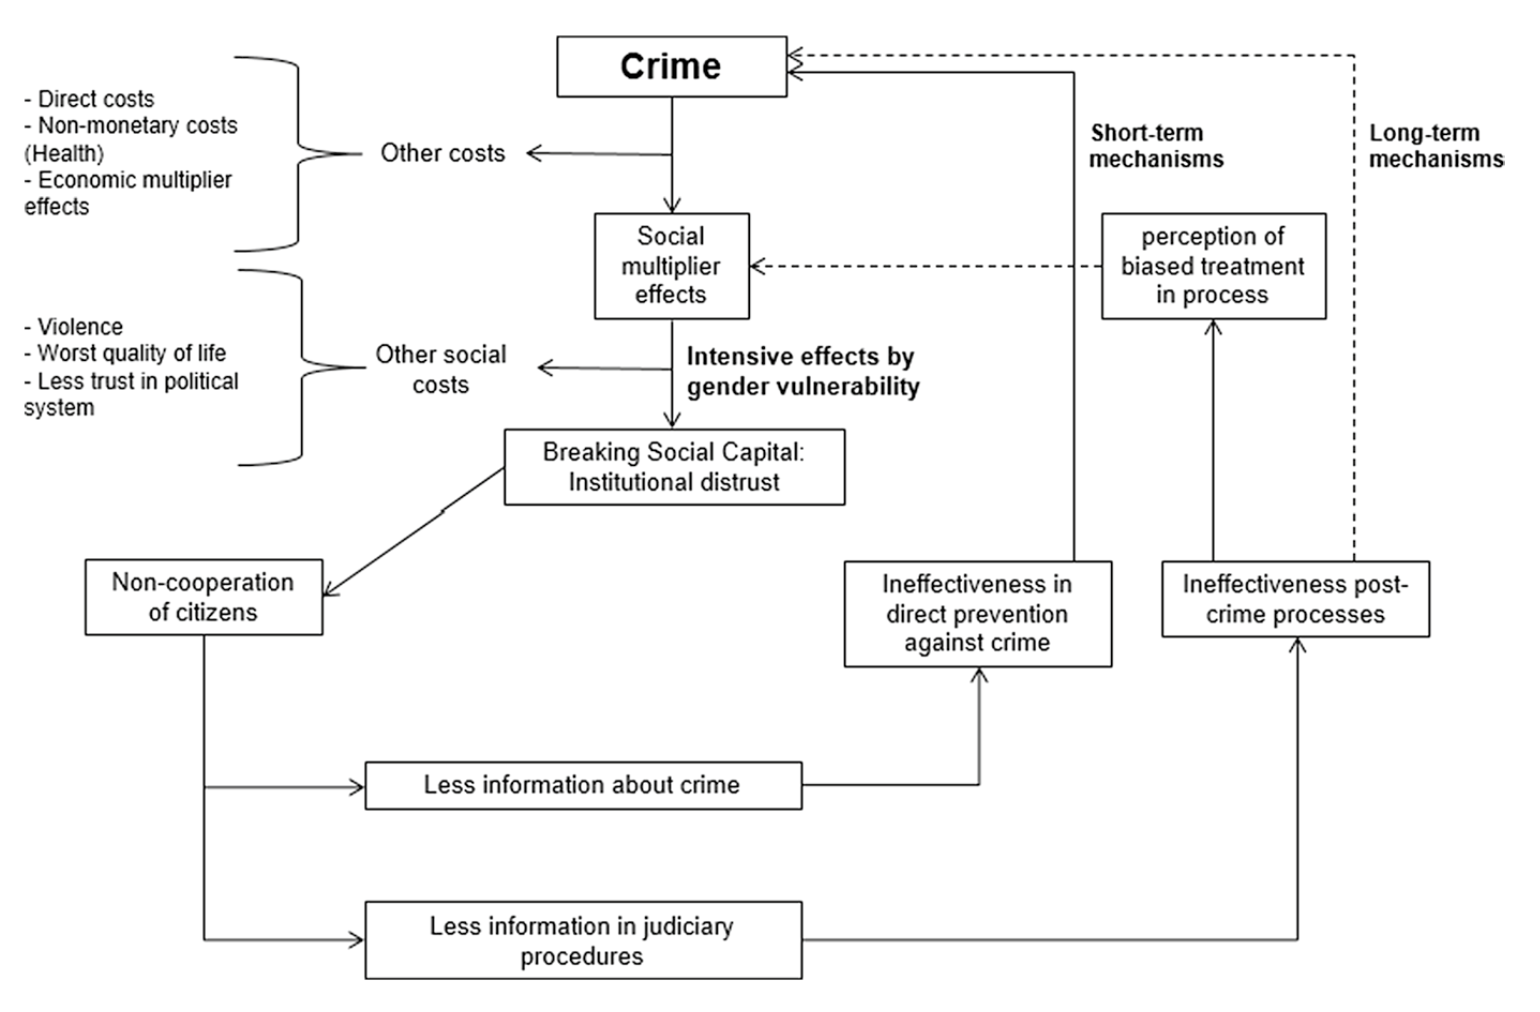
\includegraphics[width = 17cm]{plot1.png}
    \label{tab:Figura1}
\end{center}
\vspace{-0.2cm}

De tal suerte, sugiere Cozzubo et. al (\citeyear{cozzubo2021}), la actitud de los ciudadanos hacia algunas instituciones se puede volver hostil derivado de la inseguridad, tanto por la percepción de la incapacidad institucional, como por la sensación generalizada de inseguridad y las interacciones en instituciones judiciales. En consecuencia, la reducción de la cooperación ciudadano-institución y la pérdida de potenciales intercambios económicos y sociales genera una erosión del capital social, entendido como la extensión de las relaciones sociales dentro de un grupo \autocite{corbacho2015, corbacho2012, cozzubo2021, putnam1994, blanco2012, blanco2013b}.\\[-1.5em]

Bajo esta perspectiva teórica, la literatura se ha centrado en la relación negativa entre victimización y confianza institucional \autocite{blanco2012, blanco2013b}. En América Latina, diferentes estudios han dado muestra de esta relación \autocite{corbacho2015, corbacho2012}. Para Guatemala, Bateson identifica que las víctimas de delitos presentan niveles más bajos de confianza en el sistema judicial en comparación con las no víctimas \autocite{bateson2010}. Malone destaca que en países centroamericanos con altas tasas de criminalidad e instituciones de impartición de justicia deficientes, el miedo al delito disminuye la confianza el sistema judicial y en la policía \autocite{malone2010a}; por su parte, Pérez resalta que la victimización por delitos reduce la confianza en la policía civil nacional en El Salvador \autocite{corbacho2012}. Esta relación, tiene consecuencias negativas, además, en instituciones no vinculadas con la impartición de justicia o con la seguridad pública (\citeyear{cozzubo2021}). Como subraya Blanco (\citeyear{blanco2012}), se espera que, si los individuos se sienten inseguros o han sido víctimas de delitos, disminuya la probabilidad de que confíen en el conjunto de instituciones del Estado, y, particularmente, de las responsables de asegurar el orden \autocite{blanco2012, blanco2013b, weyland2003}.

\subsubsection{Crimen y confianza interpersonal}

En términos de confianza interpersonal, la literatura resalta que las personas depositan confianza en sus conciudadanos, confianza entre pares u horizontal, toda vez que estiman como probable que el Estado intervendrá (\emph{enforcement}) para resolver posibles conflictos. De esta forma, como indica Lo Iacono (\citeyear{lo_iacono2019}):

\begin{quote}
"\emph{If institutions are unable to practically prevent law-breaking, individuals’ evaluation of state’s reliability should tend to be negative and therefore social trust would not be fostered. For instance, Freitag and Bulhmann, argue that “if there is reason to suspect that the rule of law in a given country is weak, such that legal organs like the judicial system or law enforcement are unable to ensure secure contracting [...], mistrust between individuals is more likely to develop.}"
\end{quote}

Lo anterior, contribuye a la discusión en torno de la erosión de capital social, pues más allá de la reducción de la cooperación ciudadano-institución, el crimen puede conducir a la pérdida de potenciales interacciones sociales \autocite{corbacho2015, corbacho2012, cozzubo2021, putnam1994, blanco2012, blanco2013b}.

\subsubsection{Crimen y satisfacción con la democracia}

La literatura ha resaltado el efecto nocivo de la incidencia delictiva sobre la satisfacción con la democracia, pues donde se presentan altas tasas de criminalidad, las preferencias por gobiernos autoritarios se incrementan \autocite{fernandez2010, ceobanu2010, malone2014}. Un mecanismo subyacente, como indica \autocite{blanco2012, blanco2013b}, se puede deber a la frustración de expectativas sobre los resultados del sistema democrático, lo que lleve a exigir políticas de “\emph{mano dura}”. Sobre este respecto, investigaciones empíricas han encontrado que la presencia de crimen puede generar presiones para una “\emph{democradura}” \autocite{malone2014}; aunque es necesario resaltar que el mecanismo presenta problemas de endogeneidad, pues no necesariamente los individuos vinculan malos resultados con un modelo democrático, ya que la exigencia de “\emph{mano dura}” puede deberse, por ejemplo, a legados autoritarios. En general, como indican Smithey \& Malone (\citeyear{malone2014}), la literatura subraya el impacto del crimen en las actitudes políticas democráticas, encontrando una conexión entre victimización y el apoyo a la evasión del Estado de Derecho. 

\subsubsection{Crimen y desarrollo institucional en México}

Para México, Blanco (\citeyear{blanco2012, blanco2013b}) ha identificado el efecto negativo de  la criminalidad en la confianza institucional. En \emph {The Impact of Insecurity on Democracy and Trust in Institutions in Mexico}, Blanco et. al. encuentran, por medio de regresión logística ordinal (\emph{Ordinal Logistic Regression} con datos de 2004 a 2010 de la Encuesta Nacional Sobre la Inseguridad (ENSI) y del \emph{Latin American Public Opinion Project} (LAPOP), un efecto negativo robusto de la victimización por algún delito sobre la confianza en las instituciones.\\[-1.5em] 

Por su parte, Randau (\citeyear{randau2022}) ha analizado el impacto de la violencia a nivel municipal utilizando modelos de efectos fijos (\emph{Linear Fixed Effects Model}), encontrando un efecto significativo positivo entre la exposición a enfrentamientos criminales y la confianza en las fuerzas policiales federales, estatales y municipales. Asimismo, ha identificado una relación negativa entre enfrentamientos criminales y la confianza interpersonal. Igualmente, Malone (\citeyear{malone2010}) ha analizado el impacto del crimen en las actitudes de los ciudadanos hacia la democracia y su participación política, con especial foco en actitudes políticas entorno al Estado de Derecho y participación política.

\subsubsection{Victimización}

Para evaluar el impacto del crimen sobre el desarrollo institucional, democrático y social se pueden tomar dos perspectivas analíticas. Por un lado,  analizar la relación considerando la experiencia de las personas, y, por el otro, estudiar la relación entre estas variables desde las percepciones del crimen (\citeyear{malone2014}). Para este trabajo, se optará por el análisis desde la experiencia de las personas, es decir, se utilizarán datos de victimización (haber sido víctima de un delito en los últimos 12 meses). Este enfoque plantea retos para aislar el efecto del crimen sobre el desarrollo institucional, ya que no es posible asegurar que quienes son víctimas y no son víctimas de un delito sean grupos sean comparables en términos de estatus socioeconómico, años promedio de educación, exposición a medios de comunicación, y demás variables que puedan predecir las variables de respuesta planteadas. Además, como indica Blanco (\citeyear{blanco2012}), es más probable que aquellas personas victimizadas tengan una mayor experiencia en el trato con instituciones, lo que podría tener efectos tanto positivos como negativos en la evaluación que hacen de determinadas instituciones (\citeyear{blanco2012}).

\subsubsection{Contribución al conocimiento actual}

El trabajo propuesto expande la literatura revisada al incorporar al análisis una nueva serie de datos para el periodo 2012 - 2023, permitiendo así evaluar la victimización sobre la confianza institucional, la satisfacción democrática en México y la confianza interpersonal a lo largo del tiempo. Con lo que se busca identificar posibles cambios en el comportamiento de las personas derivado del dinamismo social y político, especialmente, considerando las políticas de seguridad implementadas durante el sexenio de Andrés Manuel López Obrador (2018 - 2024) y su posible impacto en el desarrollo institucional. Asimismo, el trabajo ofrece un análisis robusto para informar políticas públicas en áreas de seguridad y justicia, contribuyendo así al diseño de estrategias más efectivas para fortalecer la confianza institucional.\\[-1.5em] 

Igualmente, es de especial interés el tema en tanto que la presencia de instituciones débiles es un factor que puede limitar el crecimiento económico en los países en desarrollo \autocite{acemoglu2003, blanco2013}, y, además, conducir a periodos de inestabilidad e incertidumbre política. Como indica Blanco (\citeyear{blanco2012, blanco2013b}):

\begin{quote}
"\emph{Because Mexico can be considered a young democracy, strengthening democracy and institutions is necessary to ensure future economic development and political stability. Institutions in which citizens can trust are important for improving social and economic conditions in Mexico. If insecurity proves to have a detrimental effect on trust in institutions, then it will be necessary to pay more attention to violence issues and design policies that deal with the negative effect that crime has on institutional development.}"
\end{quote}

\vspace{-0.7cm}

%%%%%%%%
\section{Diseño empírico}

\subsection{Datos y variables} 

El análisis presentado se construyó con la serie 2010 - 2012 del \emph{Latin American Public Opinion Project} (LAPOP). Las encuestas de LAPOP son representativas a nivel nacional para adultos en edad de votar (18 años o más, abarcando 29 de los 32 estados) y cuentan con un diseño de muestra que incluye estratificación y agrupamiento. El tamaño de la muestra para cada una de las series de LAPOP incluye a alrededor de 1,500 observaciones. Las variables de la encuesta utilizada para el análisis son las siguientes:

\subsubsection{Variable independiente} 

\vspace{-0.2cm}
\begin{itemize}
\setlength{\itemsep}{0pt}%
\setlength{\parskip}{0pt}%
\item \emph{Victimización}: Ha sido usted víctima de algún acto de delincuencia en los últimos 12 meses? Es decir, \text{?`}ha sido usted víctima de un robo, hurto, agresión, fraude, chantaje, extorsión, amenazas o algún otro tipo de acto delincuencial en los últimos 12 meses?
\end{itemize}

\subsubsection{Variable dependiente} 

\vspace{-0.2cm}
\begin{itemize}
\setlength{\itemsep}{0pt}%
\setlength{\parskip}{0pt}%
\item \emph{Confianza en el presidente}: \text{?`}Hasta qué punto tiene usted confianza en el presidente?
\item \emph{Confianza a nivel municipal}: \text{?`}Hasta qué punto tiene usted confianza en su municipalidad?
\item \emph{Confianza interpersonal}: \text{?`}Diría que la gente de su comunidad es muy confiable, algo confiable, poco confiable o nada confiable?
\item \emph{Satisfacción con la democracia}: \text{?`}Usted diría que está muy satisfecho(a), satisfecho(a), insatisfecho(a) o muy insatisfecho(a) con la forma en que la democracia funciona en (país)?
\end{itemize}

\subsection{Modelo estadístico} 

Para el análisis se utilizó una regresión logística ordinal (\emph{Ordinal Logistic Regression}). La regresión logística ordinal se utiliza para modelar una variable dependiente ordinal dada una o más variables independientes. Se optó por el modelo logístico ordinal en tanto que la variable de respuesta está registrada en escala \emph{Likert}. El modelo estadístico propuesto está definido como:

\[
logit(p) = \ln\left(\frac{\text{\emph{prob}(\emph{event})}}{1 - \text{\emph{prob}(\emph{event})}}\right) = \alpha_i + \beta_1 X_1 + \beta_2 X_2 + \ldots + \beta_n X_n
\]

Donde $\ln\left(\frac{\text{\emph{prob}(\emph{event})}}{1 - \text{\emph{prob}(\emph{event})}}\right)$ es el logaritmo natural del cociente entre la probabilidad de que ocurra el evento y la probabilidad de que no ocurra (\emph{odds})\footnote{Se conoce como \emph{log-odds} logaritmo de los momios.}; $\alpha_i$ es una constantes para cada $k - 1$ categorías de la variable de respuesta ordinal; $\beta_1 X_1, \beta_2 X_2, \ldots, \beta_k X_k$ representan los efectos de las variables independientes ($X_1, X_2, \ldots, X_n$) en el \emph{log-odds} de la probabilidad; y cada $\beta_i$ es un coeficiente que mide cuánto cambia el \emph{log-odds} de la probabilidad cuando la variable independiente correspondiente cambia en una unidad.Para el análisis propuesto, el cambio en la variable independiente corresponde a un cambio en la victimización de la persona, es decir, el cambio en una variable \emph{dummy} que se computa como 1 cuando la persona fue víctima de algún delito en los últimos 12 meses y como 0 cuando no fue víctima de ningún delito.\\[-1.5em] 

Para cada modelo de regresión se asumieron los supuestos de no multicolinealidad entre las variables explicativas, es decir, que no están altamente correlacionadas. Además, se asumió el supuesto de proporcionalidad de las probabilidades (\emph{Proportional Odds Assumption}), lo que implica que la variable independiente, victimización, tiene un efecto idéntico en cada división acumulativa de la variable dependiente ordinal. Los modelos se ajustaron utilizando la función \href{https://www.rdocumentation.org/packages/ordinal/versions/2010.03-04/topics/clm}{clm()} de la librería \href{https://cran.r-project.org/web/packages/ordinal/index.html}{Ordinal} del programa estadístico \href{https://posit.co/download/rstudio-desktop/}{RStudio}.

\subsubsection{Modelo de regresión logística ordinal}

Se computarán cuatro modelos de regresión, uno para cada variable de dependiente. Para cada uno de los modelos, la variable independiente será la victimización,\footnote{En una segunda entrega se computará el modelo considerando una canasta de controles.} mientras que  la variable dependiente será alguna de las cuatro variables listadas anteriormente. En este sentido, los modelos propuestos están definidos como:

\[
logit(p) = \ln\left(\frac{\text{\emph{prob}(\emph{event})}}{1 - \text{\emph{prob}(\emph{event})}}\right) = \alpha_i + \beta_1 Victimizacion_1 + \beta_2 Year_2 
\]

Se espera que la relación entre victimización y cada variable dependiente siga el siguiente comportamiento:

\vspace{-0.2cm}
\begin{itemize}
\setlength{\itemsep}{0pt}%
\setlength{\parskip}{0pt}%
\item Haber sido víctima de algún delito disminuye la probabilidad de reportar un alto nivel de confianza en el presidente; la probabilidad de reportar un alto nivel de confianza en la municipalidad; la probabilidad de reportar un alto nivel de confianza interpersonal; y la probabilidad de reportar un alto nivel de satisfacción con la democracia.
\end{itemize}

\subsubsection{Interpretación del modelo de regresión logística ordinal} 

Así pues, el modelo de regresión logística ordinal arrojará un coeficiente $\beta$\footnote{Resultado presentado en el Cuadro I y Cuadro II} que estima el efecto de la victimización sobre la variable dependiente en cuestión, así como coeficientes para cada uno de los niveles de respuesta en que esté computada la variable dependiente\footnote{Estos coeficientes se conocen como ``umbrales'' y se presentan en las tablas del Anexo I}. Por ejemplo, sea la variable dependiente satisfacción con la democracia, computada como la respuesta a la pregunta \emph{\text{?`}Usted diría que está muy satisfecho(a), satisfecho(a), insatisfecho(a) o muy insatisfecho(a) con la forma en que la democracia funciona en México?}, el modelo arrojará una $\beta$ para cada nivel de respuesta, en este caso, muy satisfecho(a), satisfecho(a), insatisfecho(a) o muy insatisfecho(a), y una $\beta$ del efecto de la victimización. De esta forma es posible estimar el efecto que tiene la victimización en cada uno de los niveles de la variable dependiente, como, por ejemplo, estimar el efecto de la victimización sobre la probabilidad de estar muy muy insatisfecho(a) con la democracia.

\vspace{-0.4cm}

%%%%%%%%
\section{Resultados}

A continuación se presentan los resultados de los modelos de regresión ordinal. En términos de interpretación, las $\beta_i$ del modelo se entienden como el cambio en el valor esperado de la evaluación (\emph{log-odds}) por el cambio en la \emph{dummy} de  victimización, \emph{ceteris paribus} (\emph{Cuadro I: Log-odds de los modelos de regresión logística ordinal}).\\

\begin{table}[!htbp] \centering 
  \caption{Log-odds de los modelos de regresión logística ordinal} 
  \label{} 
\begin{tabular}{@{\extracolsep{5pt}}lcccc} 
\\[-1.8ex]\hline 
\hline \\[-1.8ex] 
 & \multicolumn{4}{c}{\textit{Variable dependiente:}} \\ 
\cline{2-5} 
\\[-1.8ex] & Presidente & Municipalidad & Interpersonal & Democracia \\
\\[-1.8ex] & (1) & (2) & (3) & (4)\\ 
\hline \\[-1.8ex] 
 Victimización & $-$0.358$^{***}$ & $-$0.416$^{***}$ & 0.202$^{***}$ & 0.361$^{***}$ \\ 
  & (0.029) & (0.029) & (0.028) & (0.033) \\ 
  & & & & \\ 
 2012 & 0.052 & 0.050 & 0.028 & $-$0.178$^{**}$ \\ 
  & (0.062) & (0.064) & (0.067) & (0.085) \\ 
  & & & & \\ 
 2014 & $-$0.797$^{***}$ & $-$0.287$^{***}$ & $-$0.138$^{**}$ & 0.279$^{***}$ \\ 
  & (0.064) & (0.064) & (0.067) & (0.070) \\ 
  & & & & \\ 
 2016 & $-$1.478$^{***}$ & $-$0.403$^{***}$ & 0.167$^{**}$ & 0.759$^{***}$ \\ 
  & (0.066) & (0.065) & (0.068) & (0.071) \\ 
  & & & & \\ 
 2019 & 0.753$^{***}$ & $-$0.144$^{**}$ & 0.142$^{**}$ & $-$0.126$^{*}$ \\ 
  & (0.065) & (0.064) & (0.069) & (0.070) \\ 
  & & & & \\ 
 2021 & 0.197$^{**}$ &  & 0.104 &  \\ 
  & (0.086) &  & (0.070) &  \\ 
  & & & & \\ 
 2023 & 0.807$^{***}$ & $-$0.010 & 0.126$^{*}$ & $-$0.636$^{***}$ \\ 
  & (0.064) & (0.063) & (0.067) & (0.070) \\ 
  & & & & \\ 
\hline \\[-1.8ex] 
N & 9,894 & 9,235 & 10,507 & 8,199 \\ 
Log Likelihood & $-$17,837.980 & $-$17,399.810 & $-$13,391.020 & $-$8,964.080 \\ 
\hline 
\hline \\[-1.8ex] 
\textit{Nota:}  & \multicolumn{4}{r}{$^{*}$p$<$0.1; $^{**}$p$<$0.05; $^{***}$p$<$0.01} \\ 
\end{tabular} 
\end{table}

Asimismo, se presenta la razón de probabilidades de cada uno de los coeficientes $\beta_i$ (\emph{Cuadro II: Odds ratio de los modelos de regresión logística ordinal}).\\ 

\begin{table}[!htbp] \centering 
  \caption{Odds ratio de los modelos de regresión logística ordinal} 
  \label{} 
\begin{tabular}{@{\extracolsep{5pt}}lcccc} 
\\[-1.8ex]\hline 
\hline \\[-1.8ex] 
 & \multicolumn{4}{c}{\textit{Variable dependiente:}} \\ 
\cline{2-5} 
\\[-1.8ex] & Presidente & Municipalidad & Interpersonal & Democracia \\ 
\\[-1.8ex] & (1) & (2) & (3) & (4)\\ 
\hline \\[-1.8ex] 
 Victimización & 0.699$^{***}$ & 0.660$^{***}$ & 1.224$^{***}$ & 1.435$^{***}$ \\ 
  & (0.029) & (0.029) & (0.028) & (0.033) \\ 
  & & & & \\ 
 2012 & 1.053 & 1.051 & 1.028 & 0.837$^{**}$ \\ 
  & (0.062) & (0.064) & (0.067) & (0.085) \\ 
  & & & & \\ 
 2014 & 0.450$^{***}$ & 0.750$^{***}$ & 0.871$^{**}$ & 1.322$^{***}$ \\ 
  & (0.064) & (0.064) & (0.067) & (0.070) \\ 
  & & & & \\ 
 2016 & 0.228$^{***}$ & 0.668$^{***}$ & 1.181$^{**}$ & 2.136$^{***}$ \\ 
  & (0.066) & (0.065) & (0.068) & (0.071) \\ 
  & & & & \\ 
 2019 & 2.124$^{***}$ & 0.866$^{**}$ & 1.152$^{**}$ & 0.882$^{*}$ \\ 
  & (0.065) & (0.064) & (0.069) & (0.070) \\ 
  & & & & \\ 
 2021 & 1.217$^{**}$ &  & 1.110 &  \\ 
  & (0.086) &  & (0.070) &  \\ 
  & & & & \\ 
 2023 & 2.242$^{***}$ & 0.990 & 1.134$^{*}$ & 0.529$^{***}$ \\ 
  & (0.064) & (0.063) & (0.067) & (0.070) \\ 
  & & & & \\ 
\hline \\[-1.8ex] 
N & 9,894 & 9,235 & 10,507 & 8,199 \\ 
Log Likelihood & $-$17,837.980 & $-$17,399.810 & $-$13,391.020 & $-$8,964.080 \\ 
\hline 
\hline \\[-1.8ex] 
\textit{Nota:}  & \multicolumn{4}{r}{$^{*}$p$<$0.1; $^{**}$p$<$0.05; $^{***}$p$<$0.01} \\ 
\end{tabular} 
\end{table} 

\subsection{Resultados: estimación de probabilidades}

Para facilitar la interpretación, en las siguientes secciones se tomarán las $\beta–i$ de cada modelo a fin de estimar, con datos de entrenamiento, la probabilidad de calificar a una institución en cualquier categoría de la escala de \emph{Likert} dada la condición de victimización \autocite{barlaz2024, McNulty, kurz}. En general, se podría asumir que la diferencia entre las probabilidades estimadas para personas victimizadas y no victimizadas en una determinada categoría de la variable de respuesta es un \emph{proxy} no causal del impacto de la violencia sobre la confianza institucional. Sin embargo, para este trabajo nos centraremos exclusivamente en cómo ha variado la evaluación de determinadas variables de desarrollo institucional y satisfacción con la democracia de las personas victimizadas, por lo que no utilizaremos ese \emph{proxy} al considerarlo un contraste ingenuo.\\[-1.5em] 

En concreto, como se explica en la sección \emph{Contribución al conocimiento actual}, se busca identificar posibles cambios en el comportamiento de las personas a partir del inicio del sexenio de Andrés Manuel López Obrador (2018 - 2024). En este sentido, las visualizaciones presentadas tienen una línea punteada indicando el inicio de la administración de López Obrador.

%%%%% %%%%% %%%%% %%%%%
%%%%% Interpretar las gráficas, interpretar algunos coeficientes de los modelos
%%%%% %%%%% %%%%% %%%%%

\subsubsection{Probabilidades por variable dependiente}

La evaluación de confianza institucional en el Ejecutivo federal mejoró en prácticamente todas las categorías de la pregunta \emph{\text{?`}Hasta qué punto tiene usted confianza en el presidente?} En concreto, se observa una disminución significativa, de 2016 a 2019, entre las personas que han sido víctimas de algún delito respecto de la probabilidad de responder que se tiene ``Nada'' de confianza en el presidente, como lo muestra la \emph{Figura II}.\\[-1.5em]

\vspace{-0.2cm}
\begin{center}
\emph{Figura II}. Relación entre confianza en el Ejecutivo Federal y victimización.
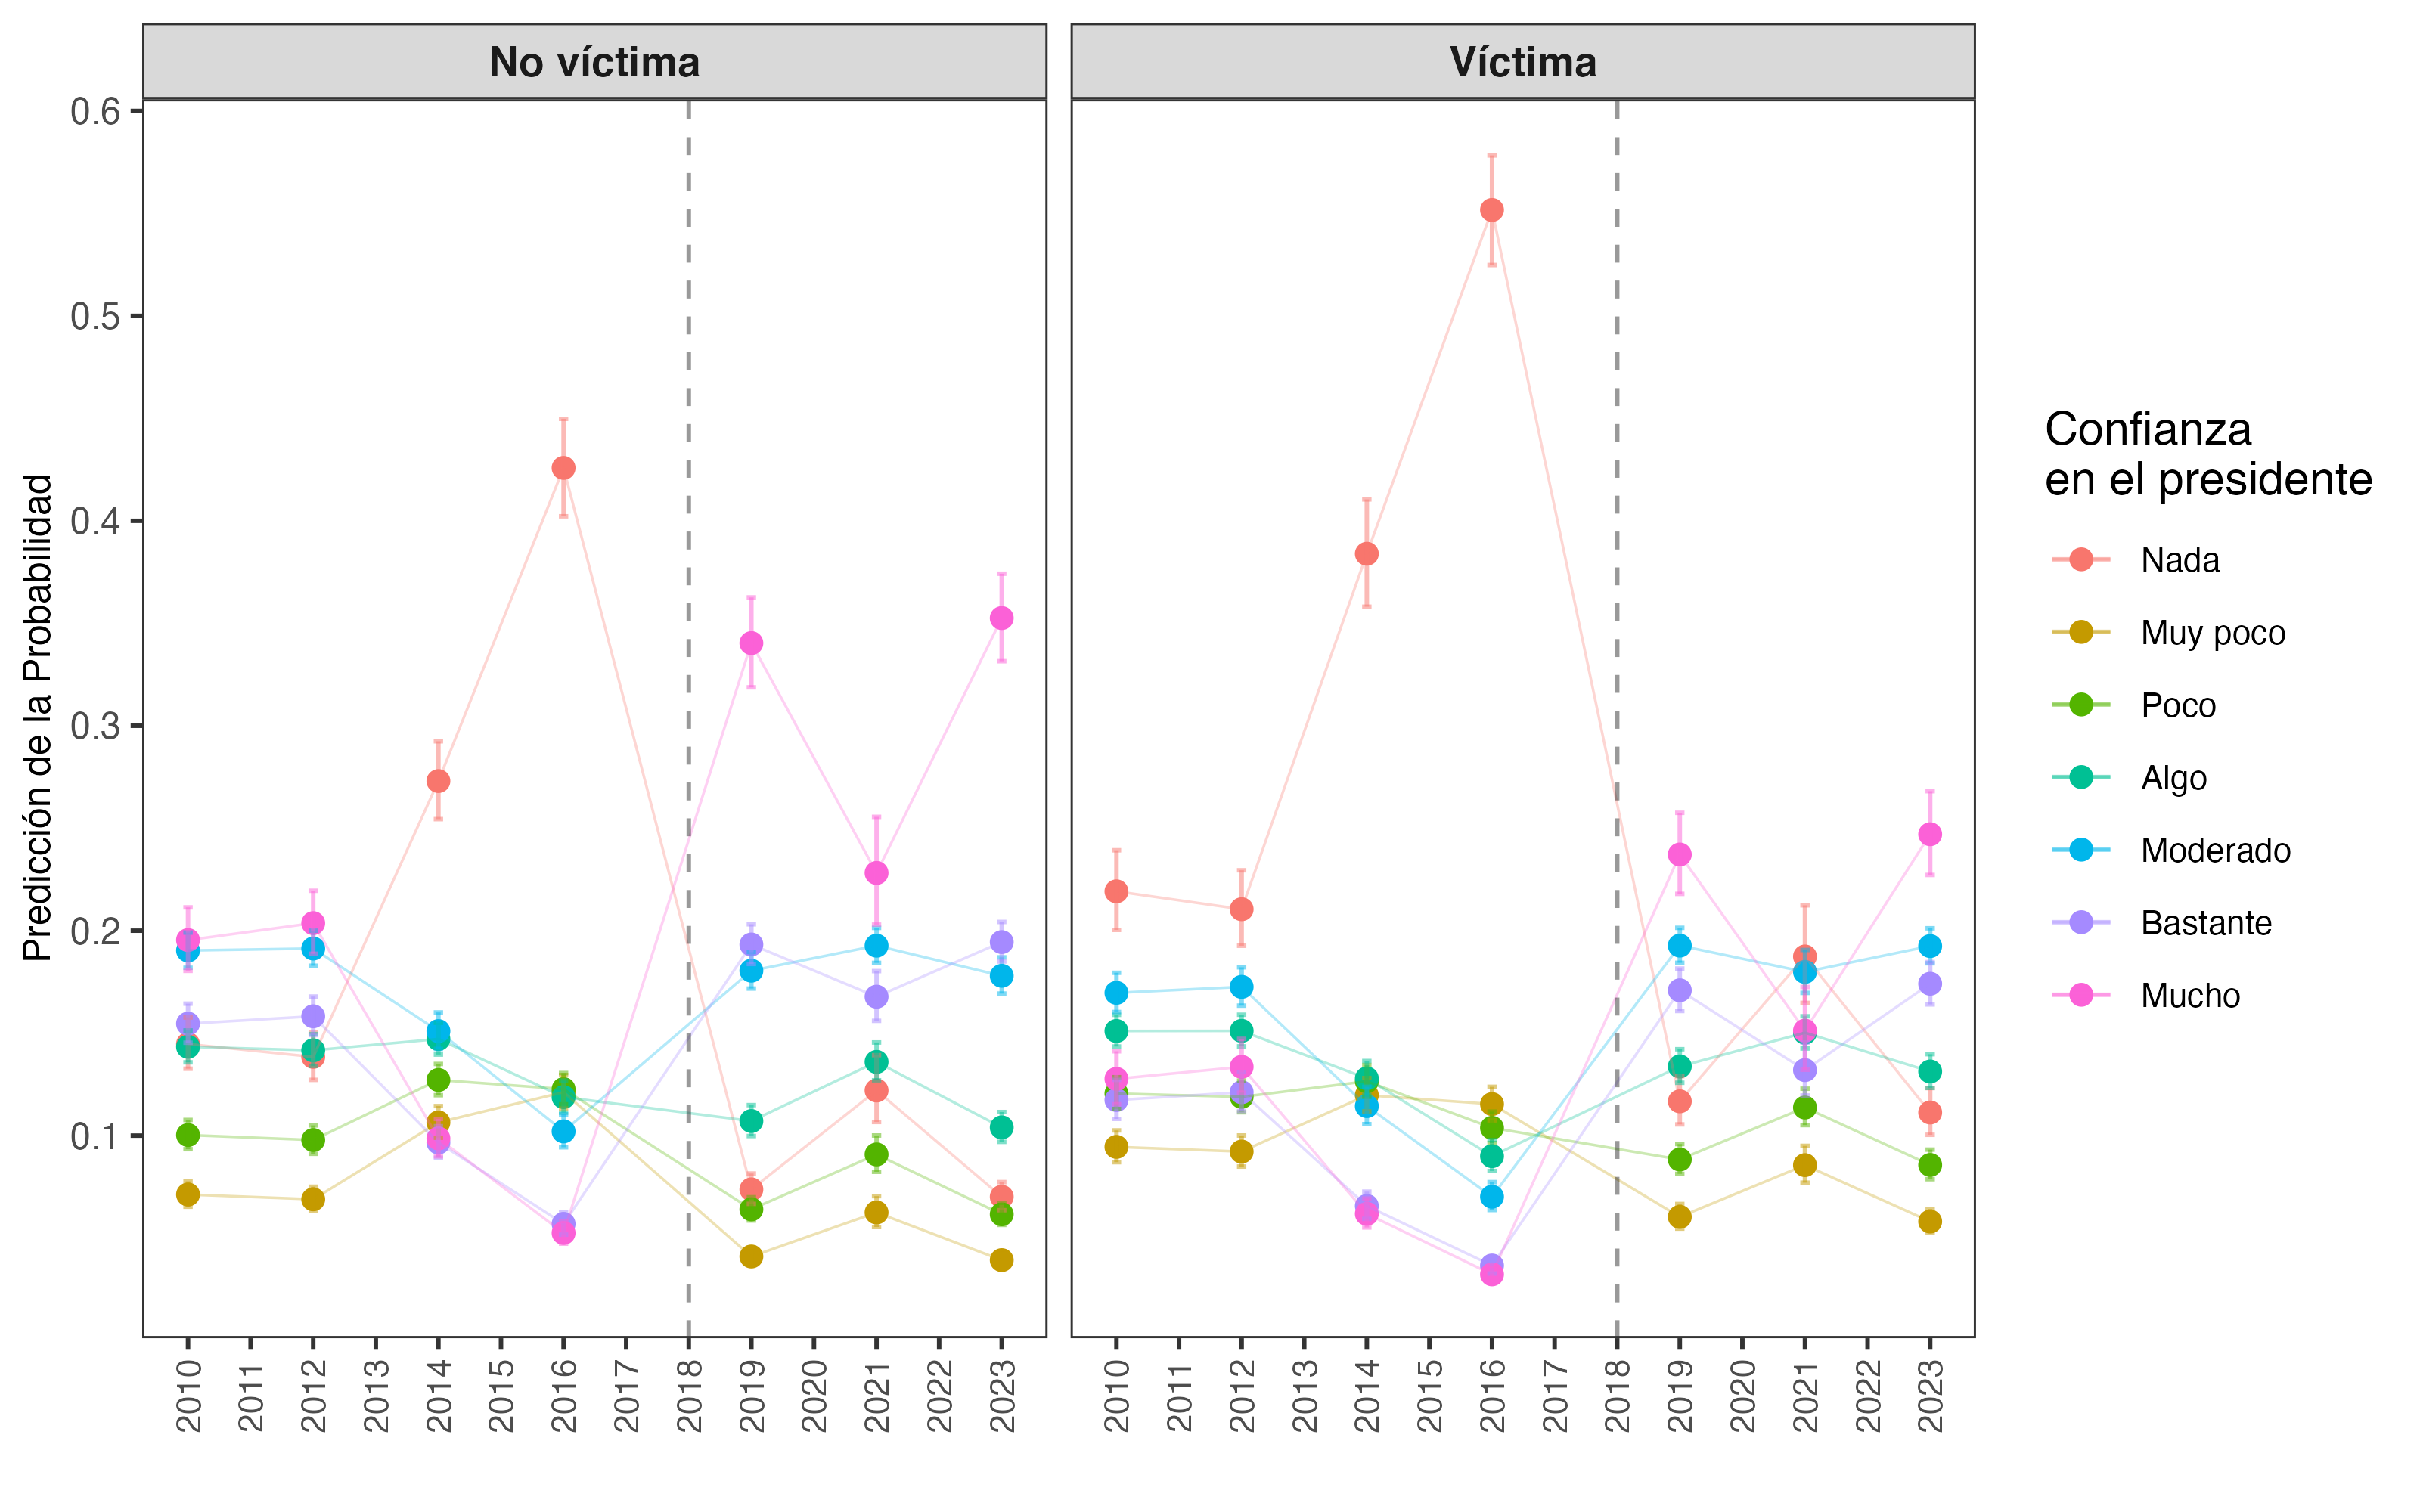
\includegraphics[width = 14cm]{plot_pres.png}
    \label{tab:Figura3}
\end{center}

Asimismo, es notoria la mejoría en la probabilidad de responder que se tiene ``Mucha confianza'' en el titular del Ejecutivo, tanto en personas victimizadas como no victimizadas. Lo anterior, contradice la relación esperada entre victimización y confianza en las instituciones del Estado, ya que la victimización disminuye la probabilidad de que confíen en el conjunto de las instituciones del Estado \autocite{blanco2012, blanco2013b, weyland2003}. Esta contradicción podría estar capturando una posible desvinculación entre confianza institucional (Ejecutivo Federal) y seguridad, lo que permitiría romper los círculos viciosos de la criminalidad que presenta Cozzubo (\citeyear{cozzubo2021}) y, como resultado, a aumentar la cooperación ciudadano-institución.\\[-1.5em]

Sin embargo, los cambios no son tan drásticos en todas las instituciones del Estado, como lo muestran las gráficas de confianza en la municipalidad. En general, para esta variable el comportamiento de las personas se ha mantenido constante, con pequeñas mejorías por categorías. Por ejemplo, ha disminuido la probabilidad de responder que se tiene ``Nada'' de confianza en la municipalidad entre las víctimas, al tiempo que ha aumentado la probabilidad de responder que se tiene ``Mucha'' confianza en la municipalidad entre personas victimizadas. Empero, la mejoría ha sido menos marcada que la recuperación de la confianza en el titular del Ejecutivo, como lo muestran la \emph{Figura III}.\\[-1.5em]

\vspace{-0.2cm}
\begin{center}
\emph{Figura III}. Relación entre confianza en la municipalidad y victimización.
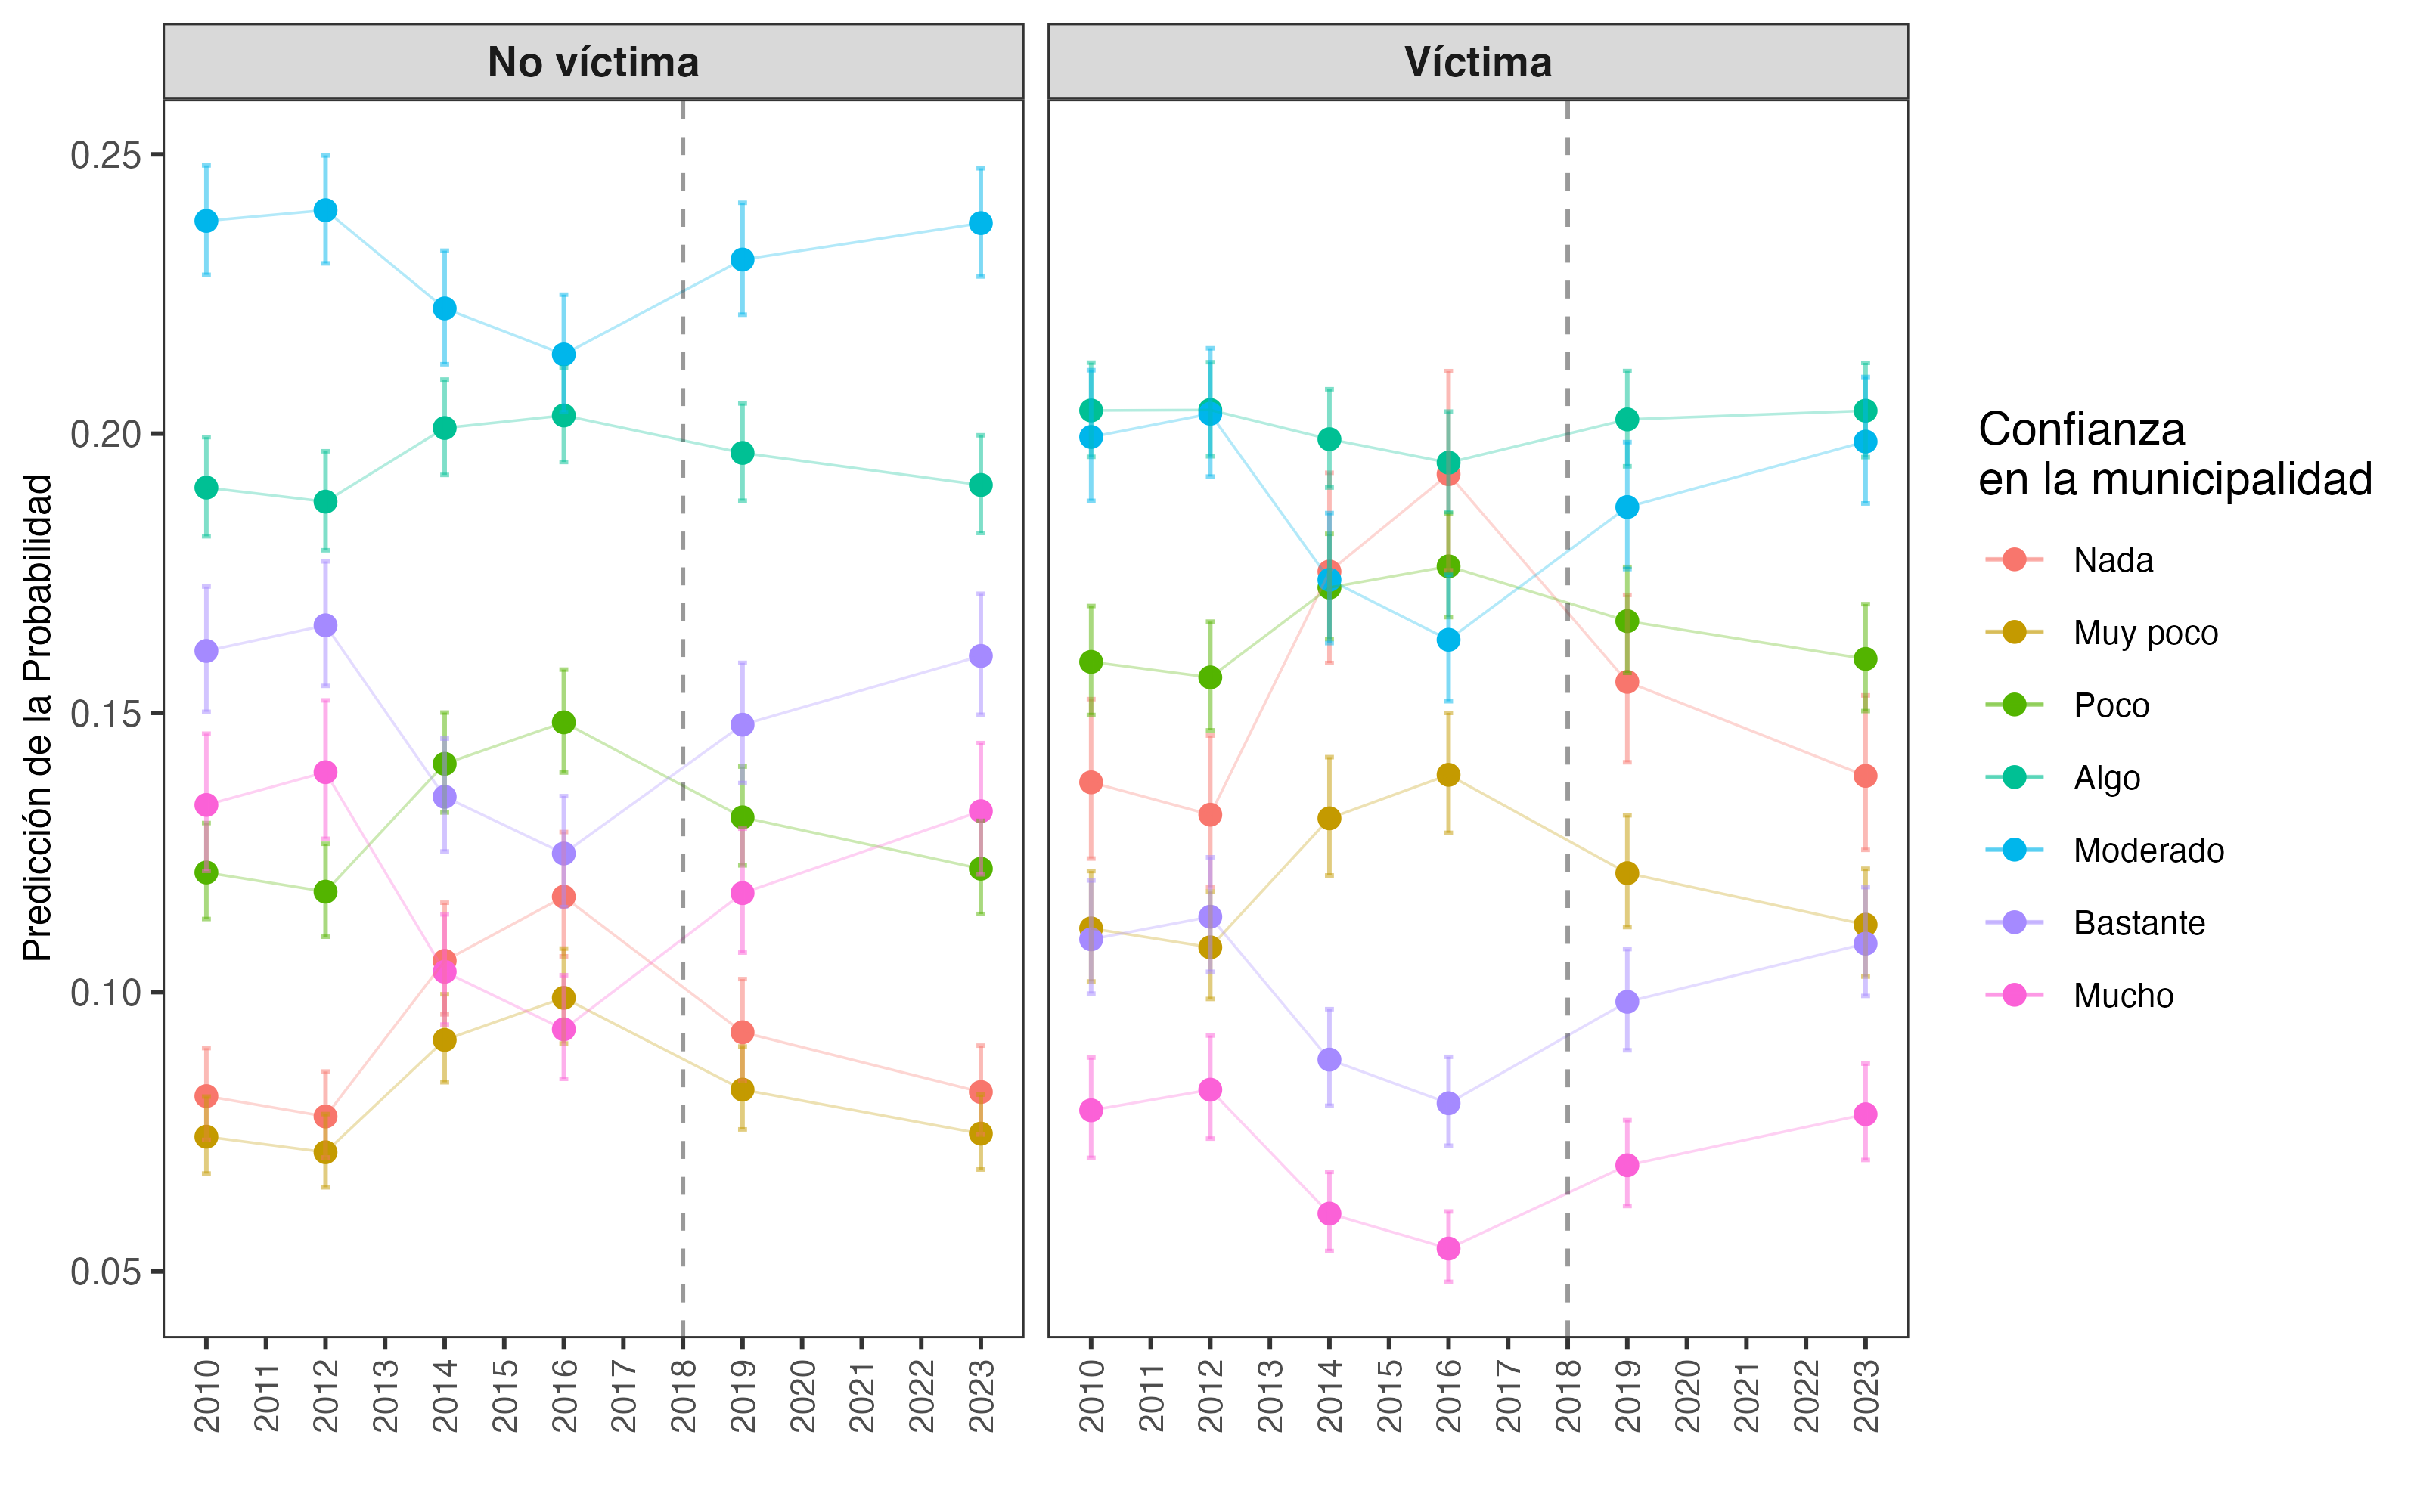
\includegraphics[width = 14cm]{plot_mun.png}
    \label{tab:Figura4}
\end{center}

Por otro lado, la \emph{Figura IV} muestra que no se ha detenido la erosión del capital social, pues la confianza interpersonal se ha mantenido en prácticamente los mismos niveles desde 2016. Esto podría indicar una posible recuperación de la confianza vertical (\emph{Figura II} y \emph{Figura III}), la cual podría tener efectos positivos a corto plazo para combatir la inseguridad y fomentar el desarrollo. Sin embargo, este avance ocurre en un contexto de estancamiento de la confianza interpersonal, lo que podría operar en sentido contrario.\\[-1.5em]

En este sentido, es relevante destacar que la limitada confianza interpersonal restringe el número de intercambios sociales y económicos potenciales, y con ello reduce las oportunidades de implementar políticas públicas efectivas basadas en la comunidad para enfrentar la delincuencia. Esta situación plantea un desafío significativo en términos de políticas, ya que la interacción social y la cooperación son fundamentales para el éxito de las estrategias de desarrollo y seguridad.\\[-1.5em]

\vspace{-0.2cm}
\begin{center}
\emph{Figura IV}. Relación entre confianza interpersonal y victimización.
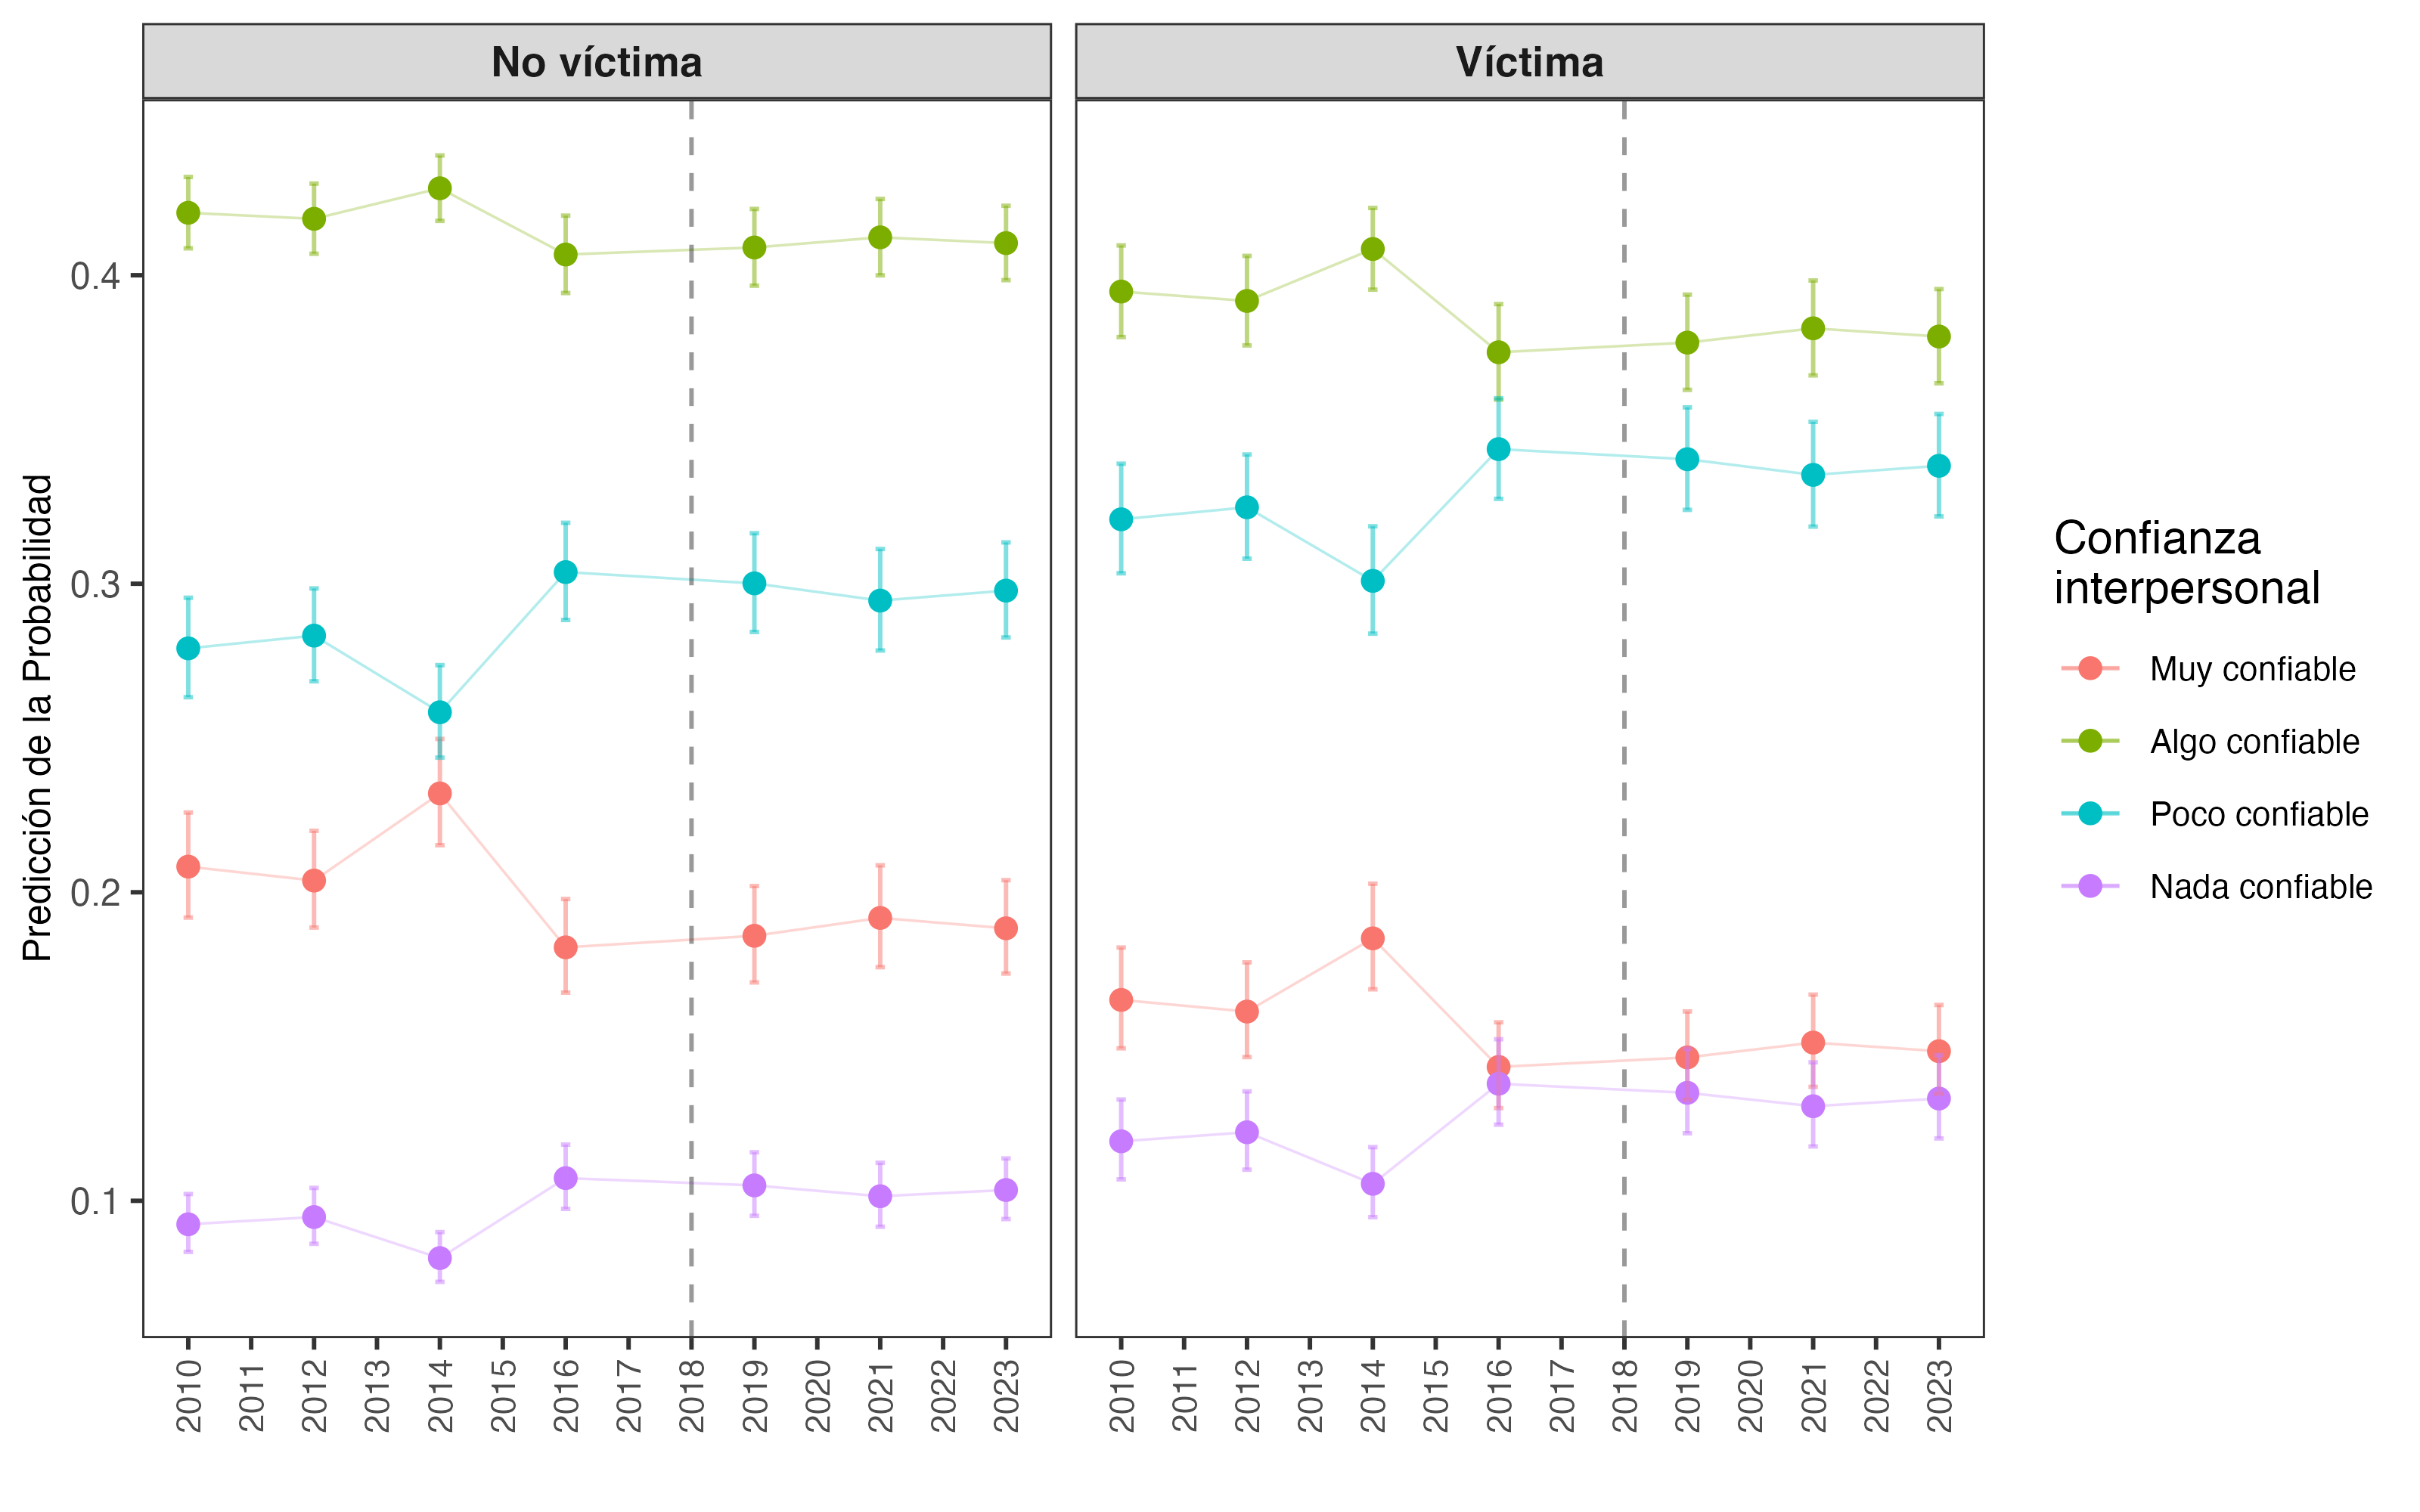
\includegraphics[width = 14cm]{plot_peer.png}
    \label{tab:Figura5}
\end{center}

En lo referente a la satisfacción con la democracia (\emph{Figura V}), se resalta una mejoría de 2016 a 2019 en la probabilidad de responder como “Satisfecho” a la pregunta \emph{¿Usted diría que está muy satisfecho(a), satisfecho(a), insatisfecho(a) o muy insatisfecho(a) con la forma en que la democracia funciona en México?} de LAPOP. Esta mejoría se observa tanto en víctimas como en no víctimas, lo que sugiere un incremento general en la satisfacción con la democracia en este período.\\[-1.5em]

Estos resultados están en línea con la recuperación de la confianza vertical mencionada anteriormente (\emph{Figura II} y \emph{Figura III}). La mejoría en la satisfacción democrática puede estar vinculada a la percepción de una mayor efectividad y legitimidad de las instituciones democráticas, lo cual, a su vez, puede estar asociado con el aumento de la confianza en las autoridades y el sistema político.\\[-1.5em]

\begin{center}
\emph{Figura V}. Relación entre satisfacción con la democracia y victimización.
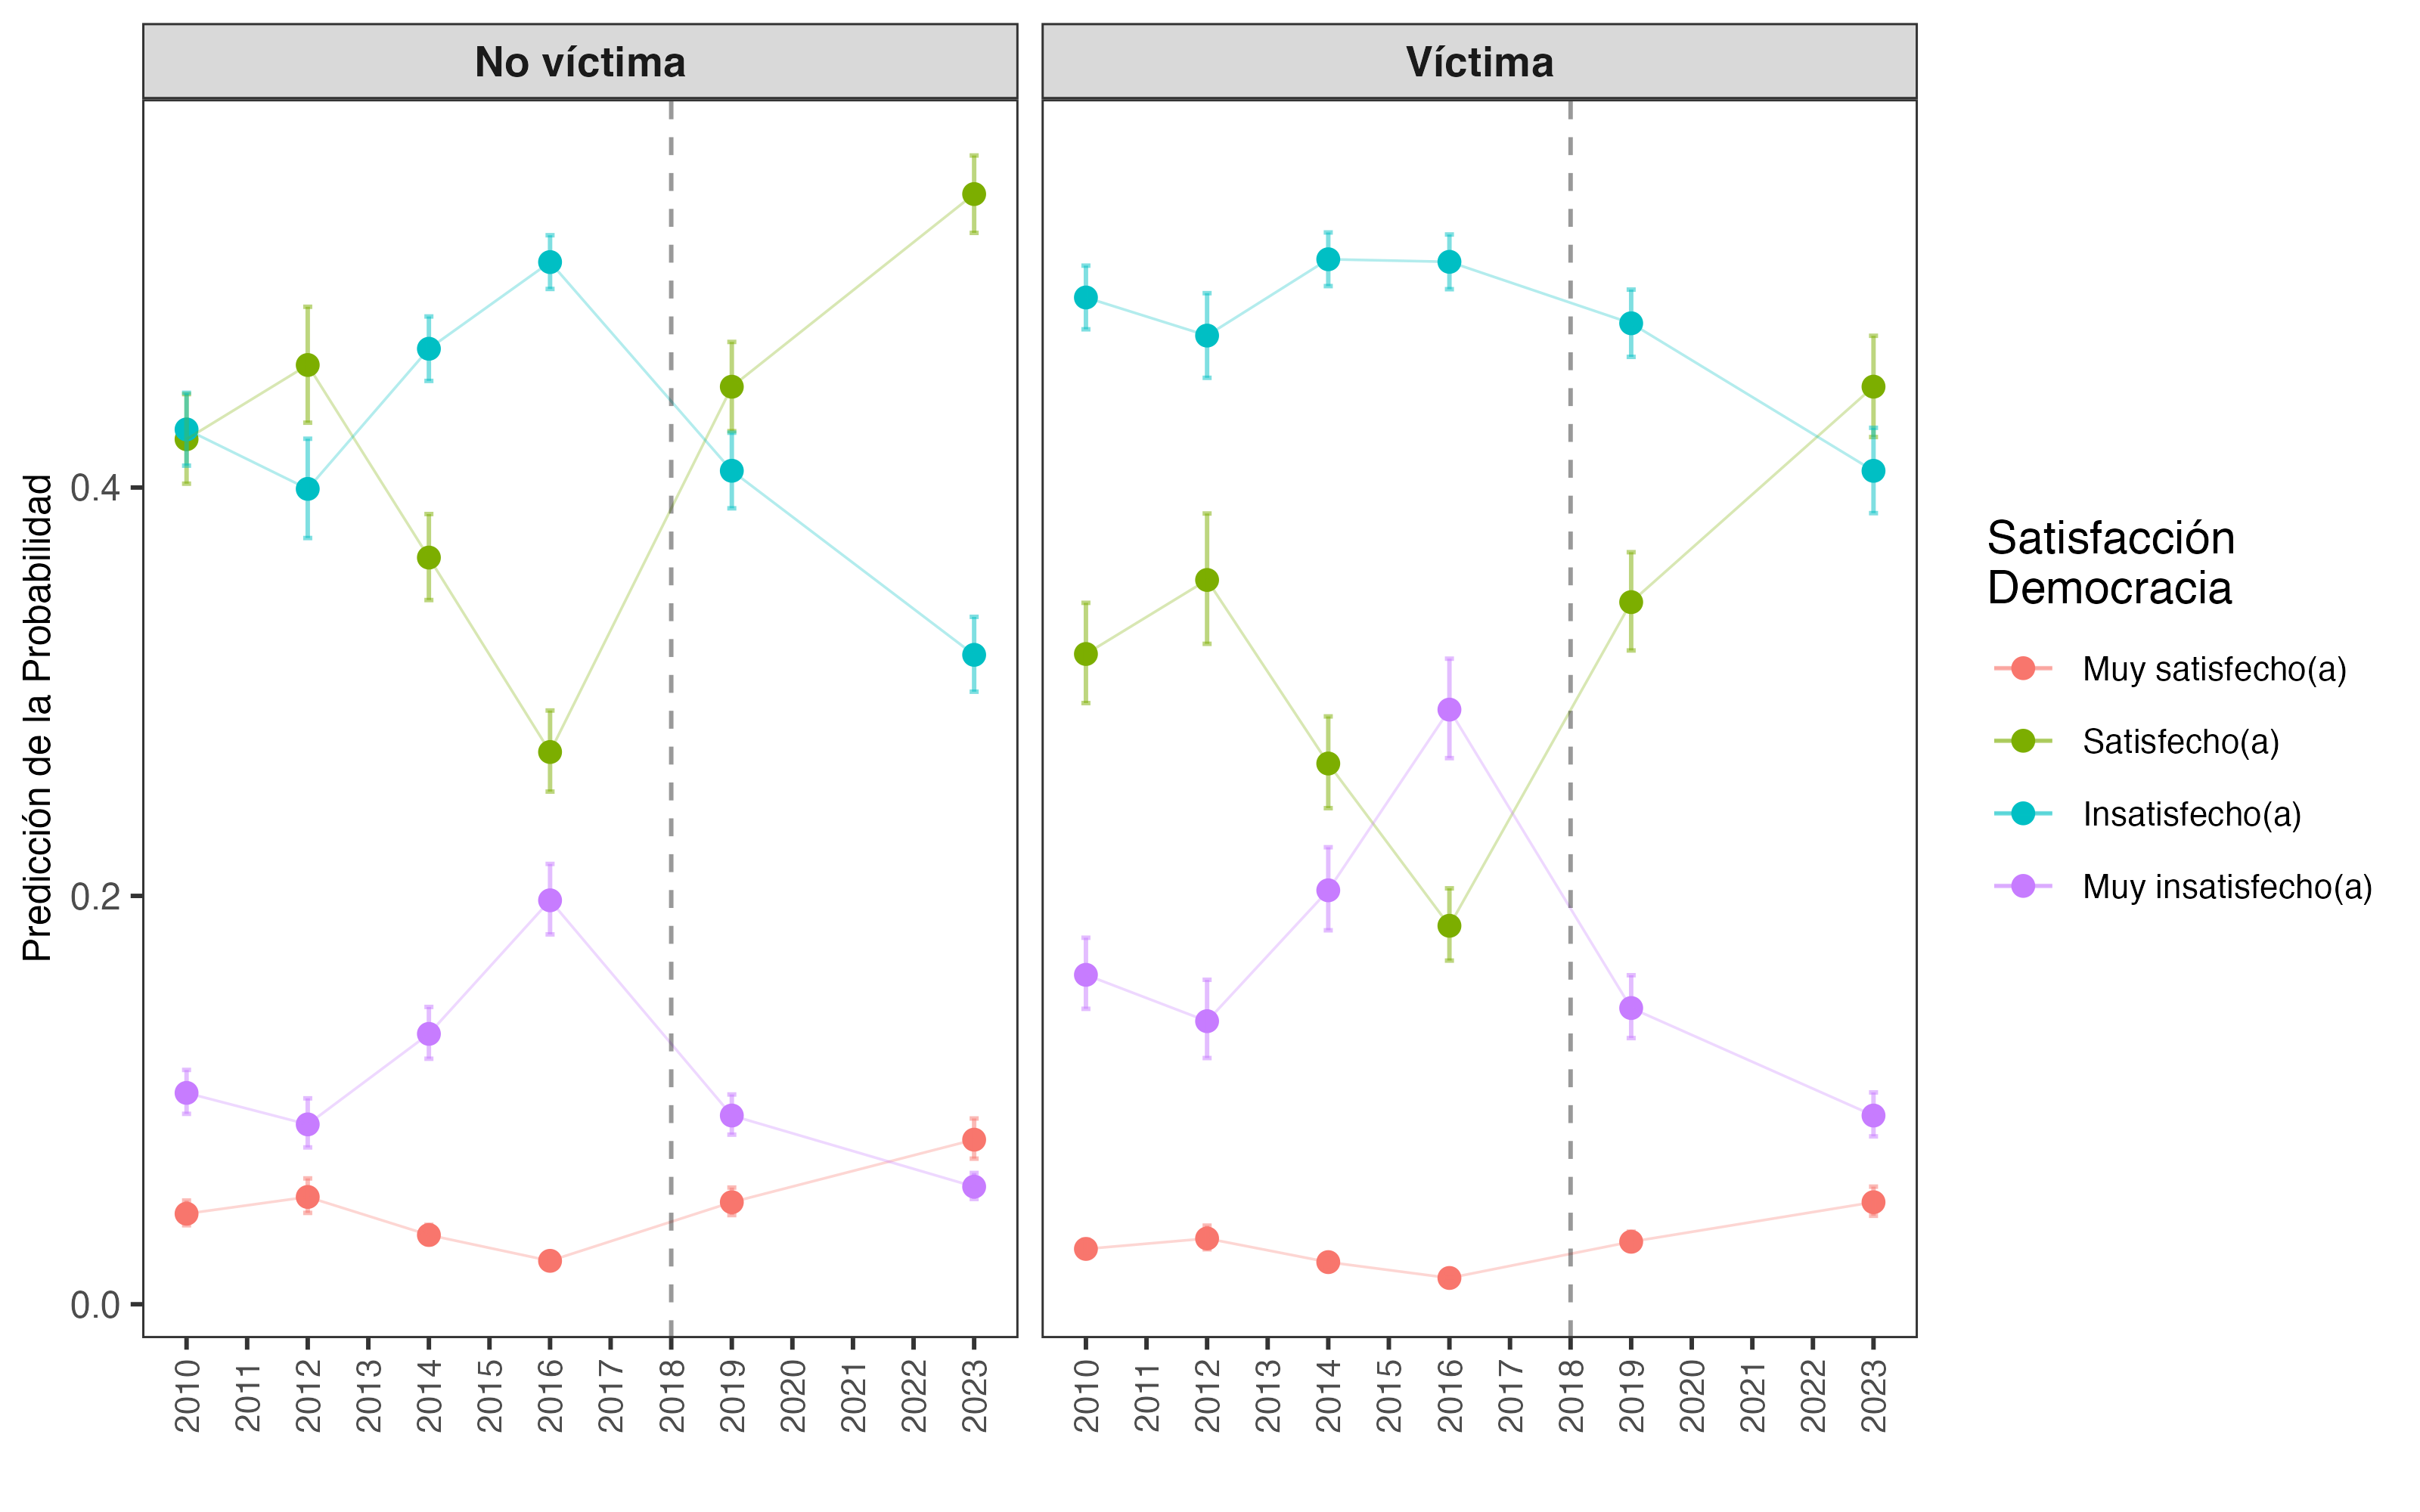
\includegraphics[width = 14cm]{plot_dem.png}
    \label{tab:Figura6}
\end{center}

\vspace{-1.5cm}

%%%%%%%%
\section{Conclusiones y discusión}

\subsection{Limitaciones}

Los resultados deben tomarse con precaución ya que no se pueden derivar inferencias causales de los mismos, ni permiten hacer un análisis a nivel de subgrupos. Asimismo, no sería correcta la comparación entre víctimas y no víctimas en tanto que las características observables y no observables de las personas “tratadas” y “no tratadas” pueden variar por variables como los patrones de movilidad, la aversión al riesgo y el nivel socioeconómico. En consecuencia, la variable de victimización podría estar registrando una suerte de “autoselección”, por lo que la comparación entre estos dos grupos sería un simple contraste ingenuo. \\[-1.5em]

Además, para tener una mayor precisión en el análisis sería conveniente incorporar posibles variables explicativas, como el nivel de ingreso, la región geográfica y los años de escolarización, así como controlar por posibles variables predictoras de la variable de respuesta.\\[-1.5em]

Igualmente, sería de utilidad explorar posibles análisis causales para identificar cómo la victimización influye en el desarrollo institucional y en el capital social de un país \autocite{corbacho2015, corbacho2012, cozzubo2021, putnam1994, blanco2012, blanco2013b}. Estos caminos podrían incluir métodos de efectos fijos \emph{Two-way Fixed Effects} para remover cualquier sesgo por variables omitidas que tengan la característica de ser constantes a través del tiempo para cada unidad de análisis, pero que varían entre unidades. Lo anterior sería posible agrupando por los estratos primarios de muestreo del LAPOP.

\vspace{-0.4cm}

%%%%%%%%
\section{Anexo I}

% Table created by stargazer v.5.2.3 by Marek Hlavac, Social Policy Institute. E-mail: marek.hlavac at gmail.com
% Date and time: Thu, May 30, 2024 - 23:46:34
\begin{table}[!htbp] \centering 
  \caption{Threshold Coefficients: Confianza en el presidente} 
\begin{tabular}{@{\extracolsep{2pt}} cccccc} 
\\[-1.8ex]\hline 
\hline \\[-1.8ex] 
Nada\textbar Muy poco & Muy poco\textbar Poco & Poco\textbar Algo & Algo\textbar Moderado & Moderado\textbar Bastante & Bastante\textbar Mucho \\ 
\hline \\[-1.8ex] 
$-1.524$ & $-1.036$ & $-0.518$ & $0.091$ & $0.872$ & $1.668$ \\ 
\hline \\[-1.8ex] 
\end{tabular} 
\end{table} 

% Table created by stargazer v.5.2.3 by Marek Hlavac, Social Policy Institute. E-mail: marek.hlavac at gmail.com
% Date and time: Thu, May 30, 2024 - 23:46:34
\begin{table}[!htbp] \centering 
  \caption{Threshold Coefficients: Confianza en la municipalidad} 
\begin{tabular}{@{\extracolsep{2pt}} cccccc} 
\\[-1.8ex]\hline 
\hline \\[-1.8ex] 
Nada\textbar Muy poco & Muy poco\textbar Poco & Poco\textbar Algo & Algo\textbar Moderado & Moderado\textbar Bastante & Bastante\textbar Mucho \\ 
\hline \\[-1.8ex] 
$-2.130$ & $-1.398$ & $-0.666$ & $0.163$ & $1.167$ & $2.164$ \\ 
\hline \\[-1.8ex] 
\end{tabular} 
\end{table} 

% Table created by stargazer v.5.2.3 by Marek Hlavac, Social Policy Institute. E-mail: marek.hlavac at gmail.com
% Date and time: Thu, May 30, 2024 - 23:46:34
\begin{table}[!htbp] \centering 
  \caption{Threshold Coefficients: Confianza interpersonal} 
\begin{tabular}{@{\extracolsep{2pt}} ccc} 
\\[-1.8ex]\hline 
\hline \\[-1.8ex] 
Muy confiable\textbar Algo confiable & Algo confiable\textbar Poco confiable & Poco confiable\textbar Nada confiable \\ 
\hline \\[-1.8ex] 
$-1.478$ & $0.383$ & $2.142$ \\ 
\hline \\[-1.8ex] 
\end{tabular} 
\end{table} 

% Table created by stargazer v.5.2.3 by Marek Hlavac, Social Policy Institute. E-mail: marek.hlavac at gmail.com
% Date and time: Thu, May 30, 2024 - 23:46:34
\begin{table}[!htbp] \centering 
  \caption{Threshold Coefficients: Satisfacción con la democracia} 
\begin{tabular}{@{\extracolsep{2pt}} ccc} 
\\[-1.8ex]\hline 
\hline \\[-1.8ex] 
Muy satisfecho(a)\textbar Satisfecho(a) & Satisfecho(a)\textbar Insatisfecho(a) & Insatisfecho(a)\textbar Muy insatisfecho(a) \\ 
\hline \\[-1.8ex] 
$-3.325$ & $-0.383$ & $1.903$ \\ 
\hline \\[-1.8ex] 
\end{tabular} 
\end{table} 

\newpage

\begin{center}
Relación entre confianza en el Ejecutivo Federal y victimización.
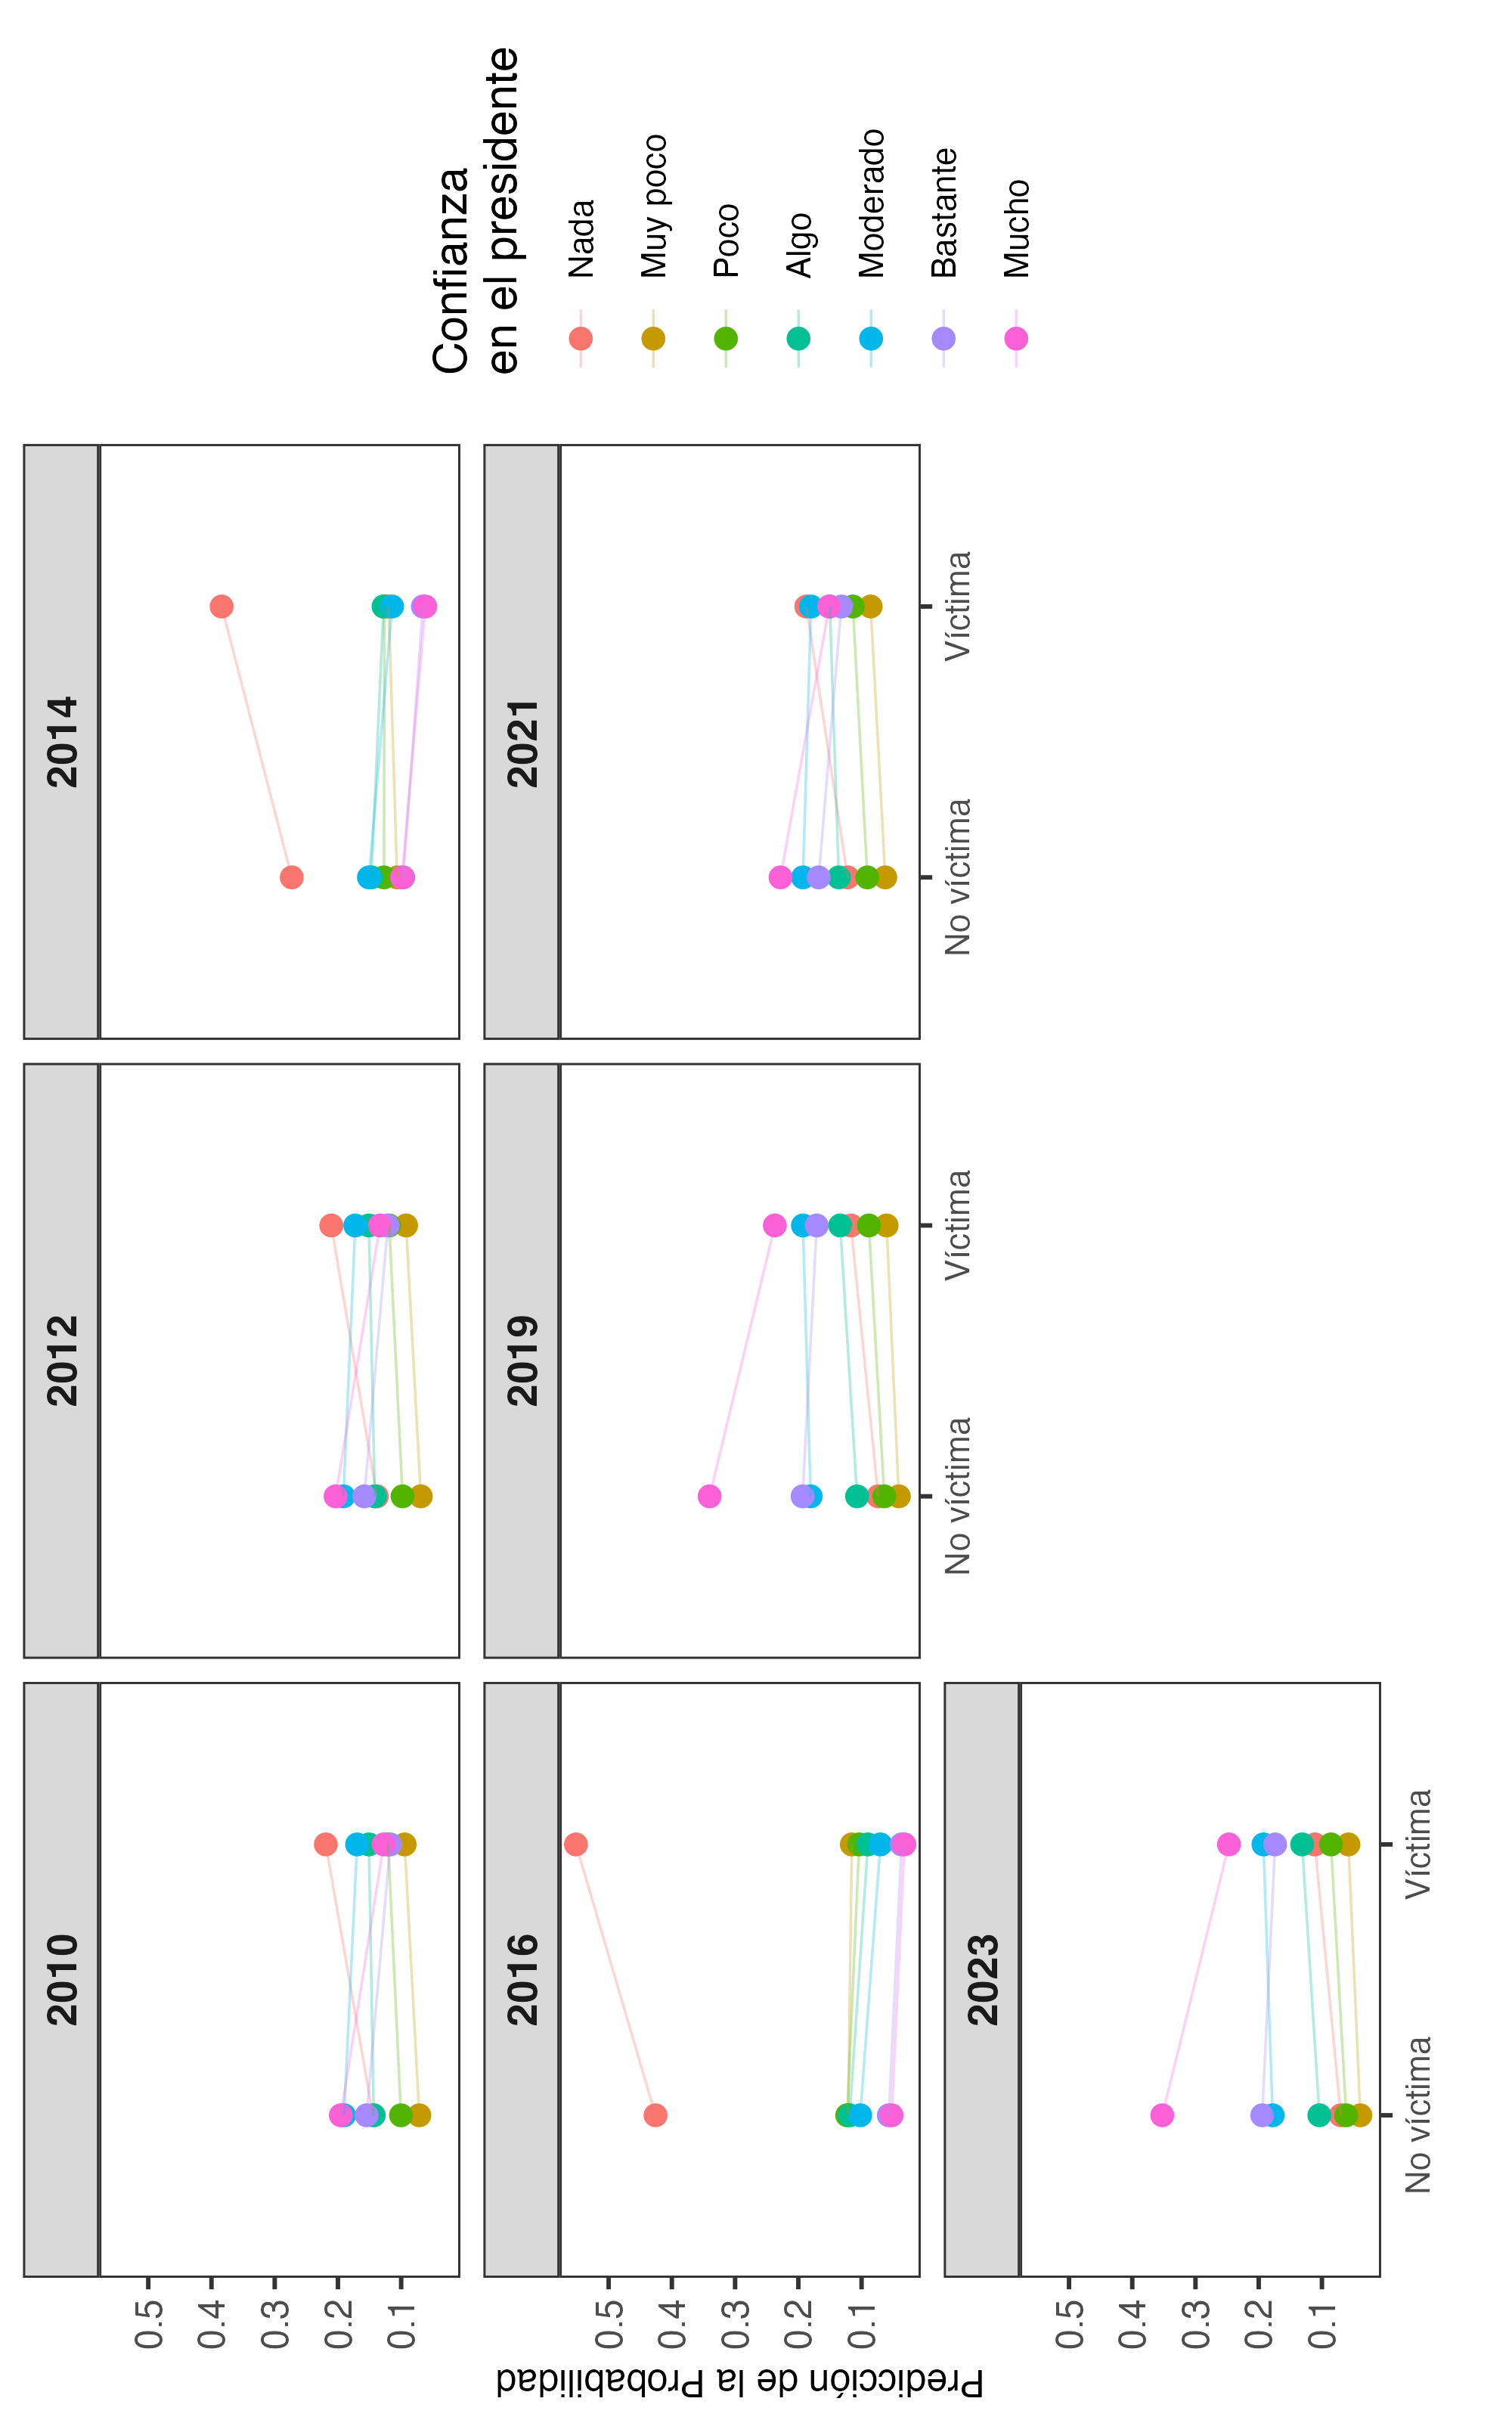
\includegraphics[width = 13cm]{plot_pres_03.png}
    \label{tab:plot3}
\end{center}

\newpage

\begin{center}
Relación entre confianza en la municipalidad y victimización.
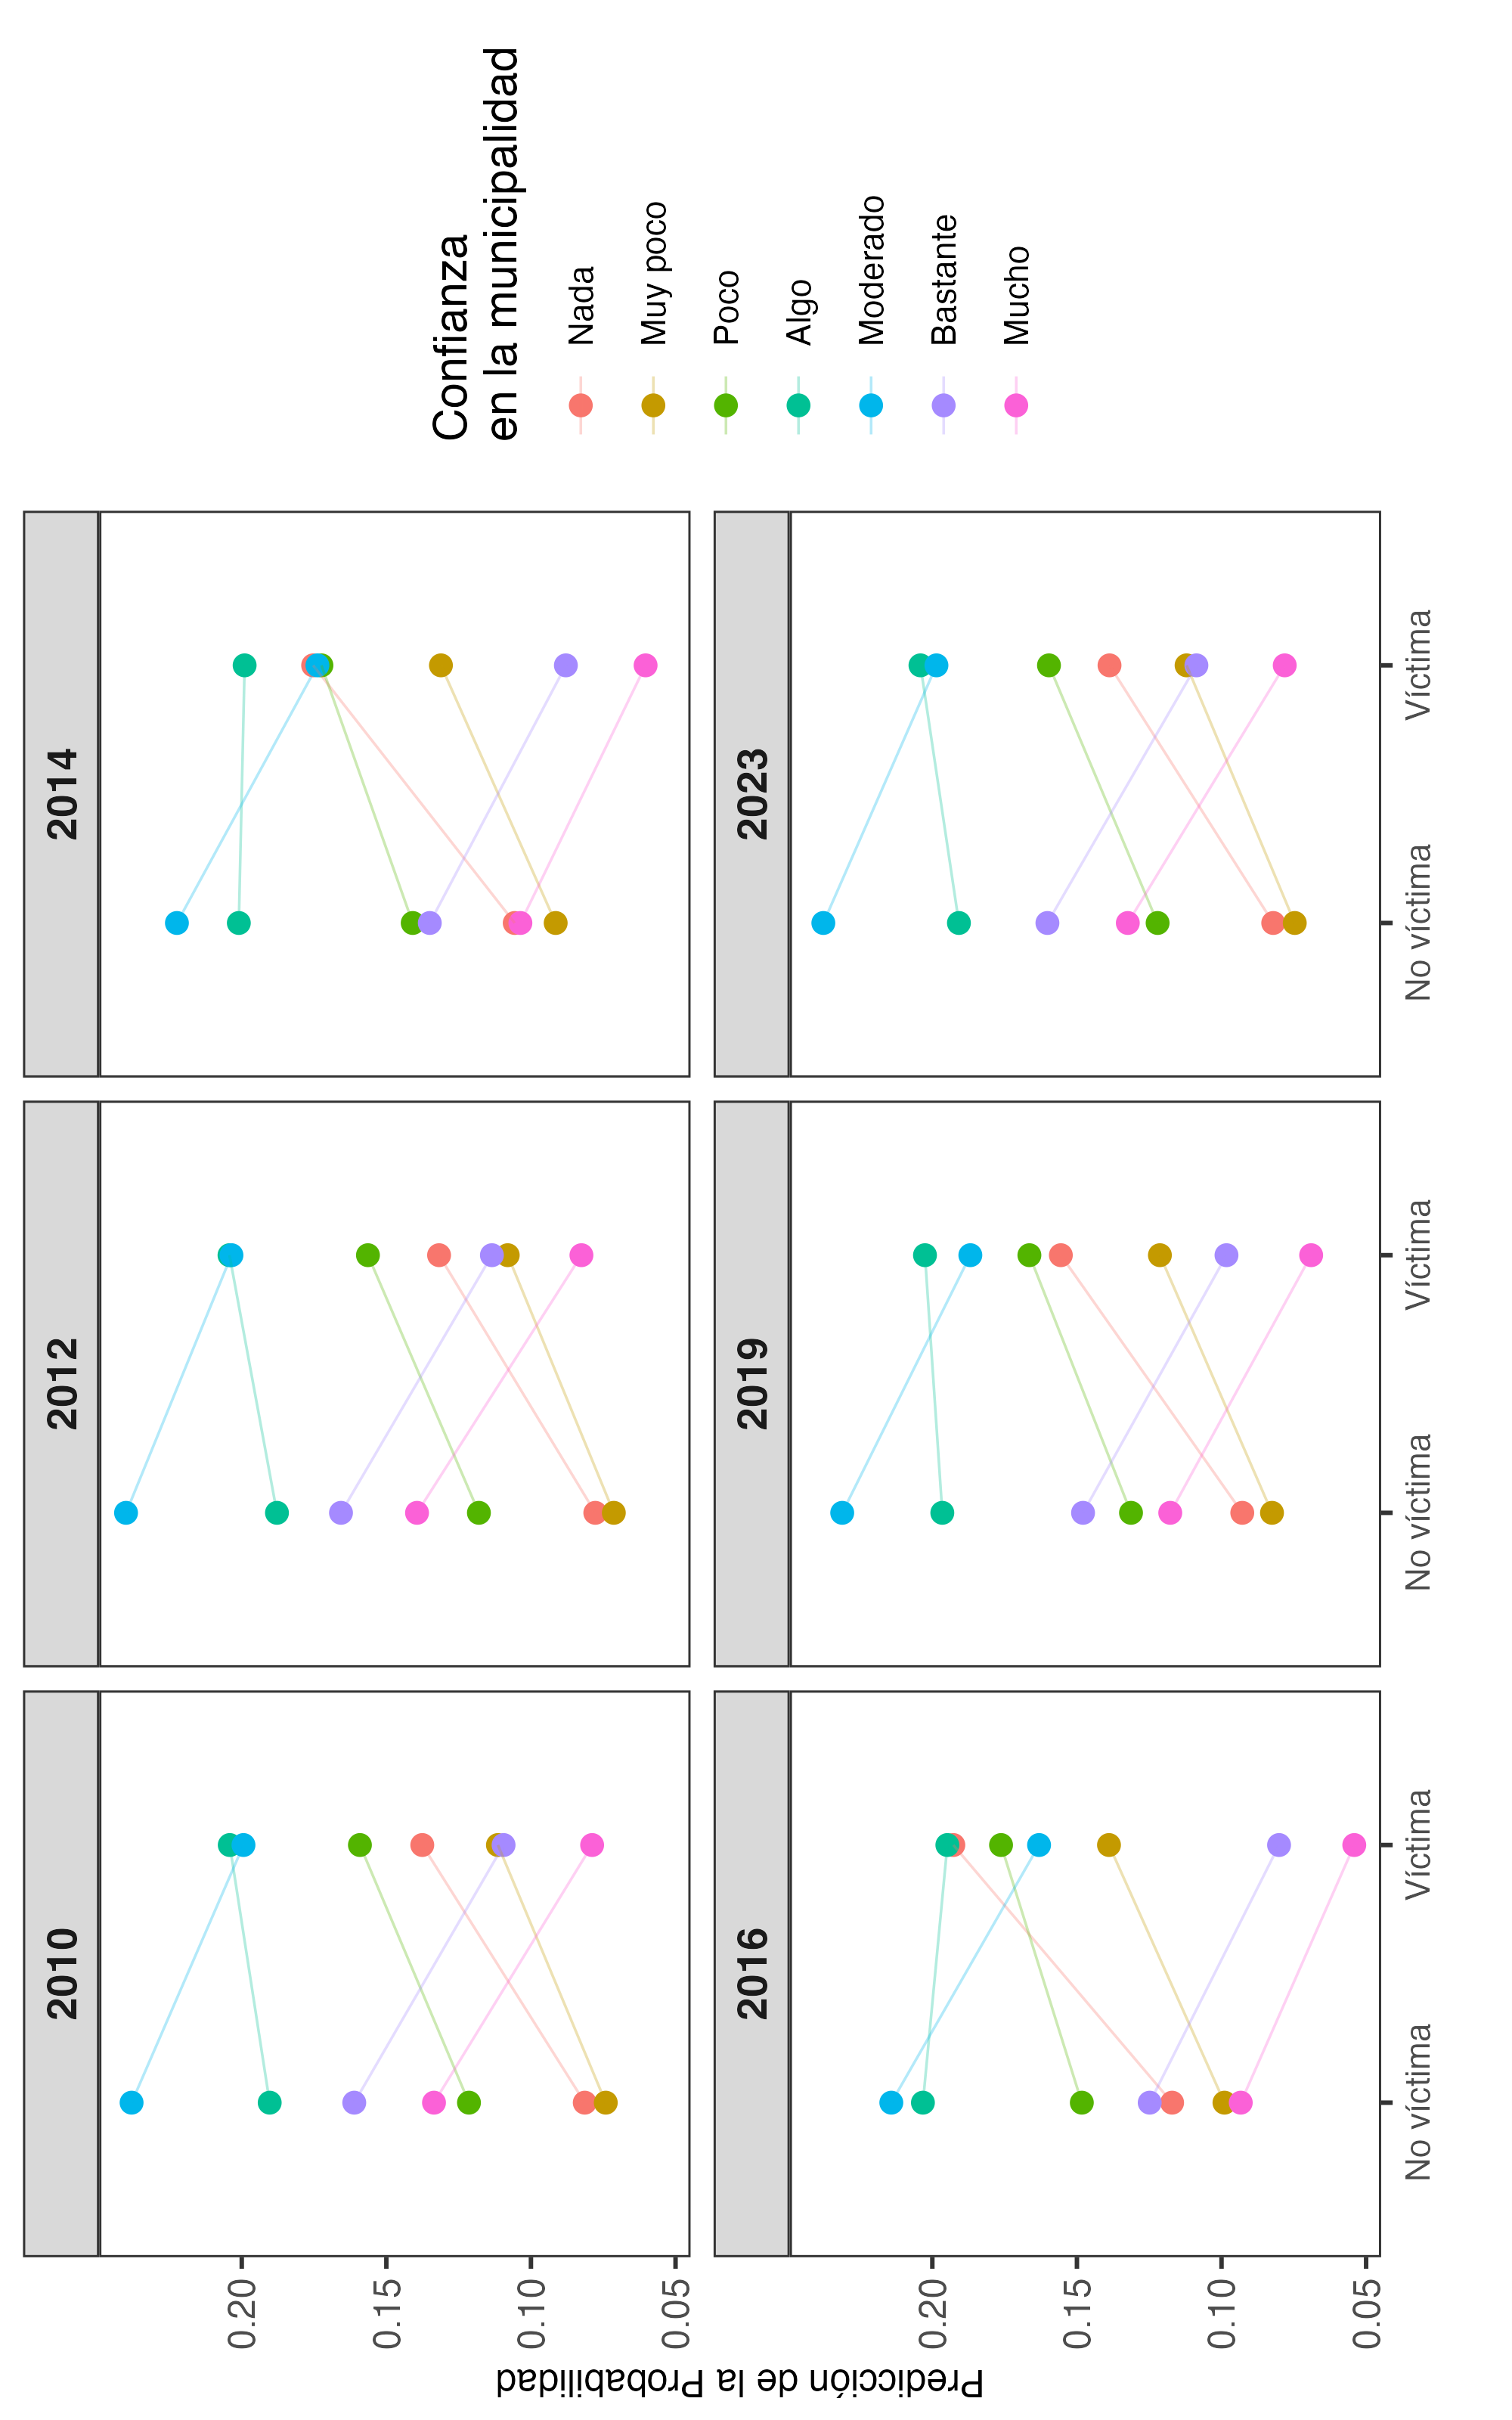
\includegraphics[width = 13cm]{plot_mun_03.png}
    \label{tab:plot4}
\end{center}

\newpage

\begin{center}
Relación entre confianza interpersonal y victimización.
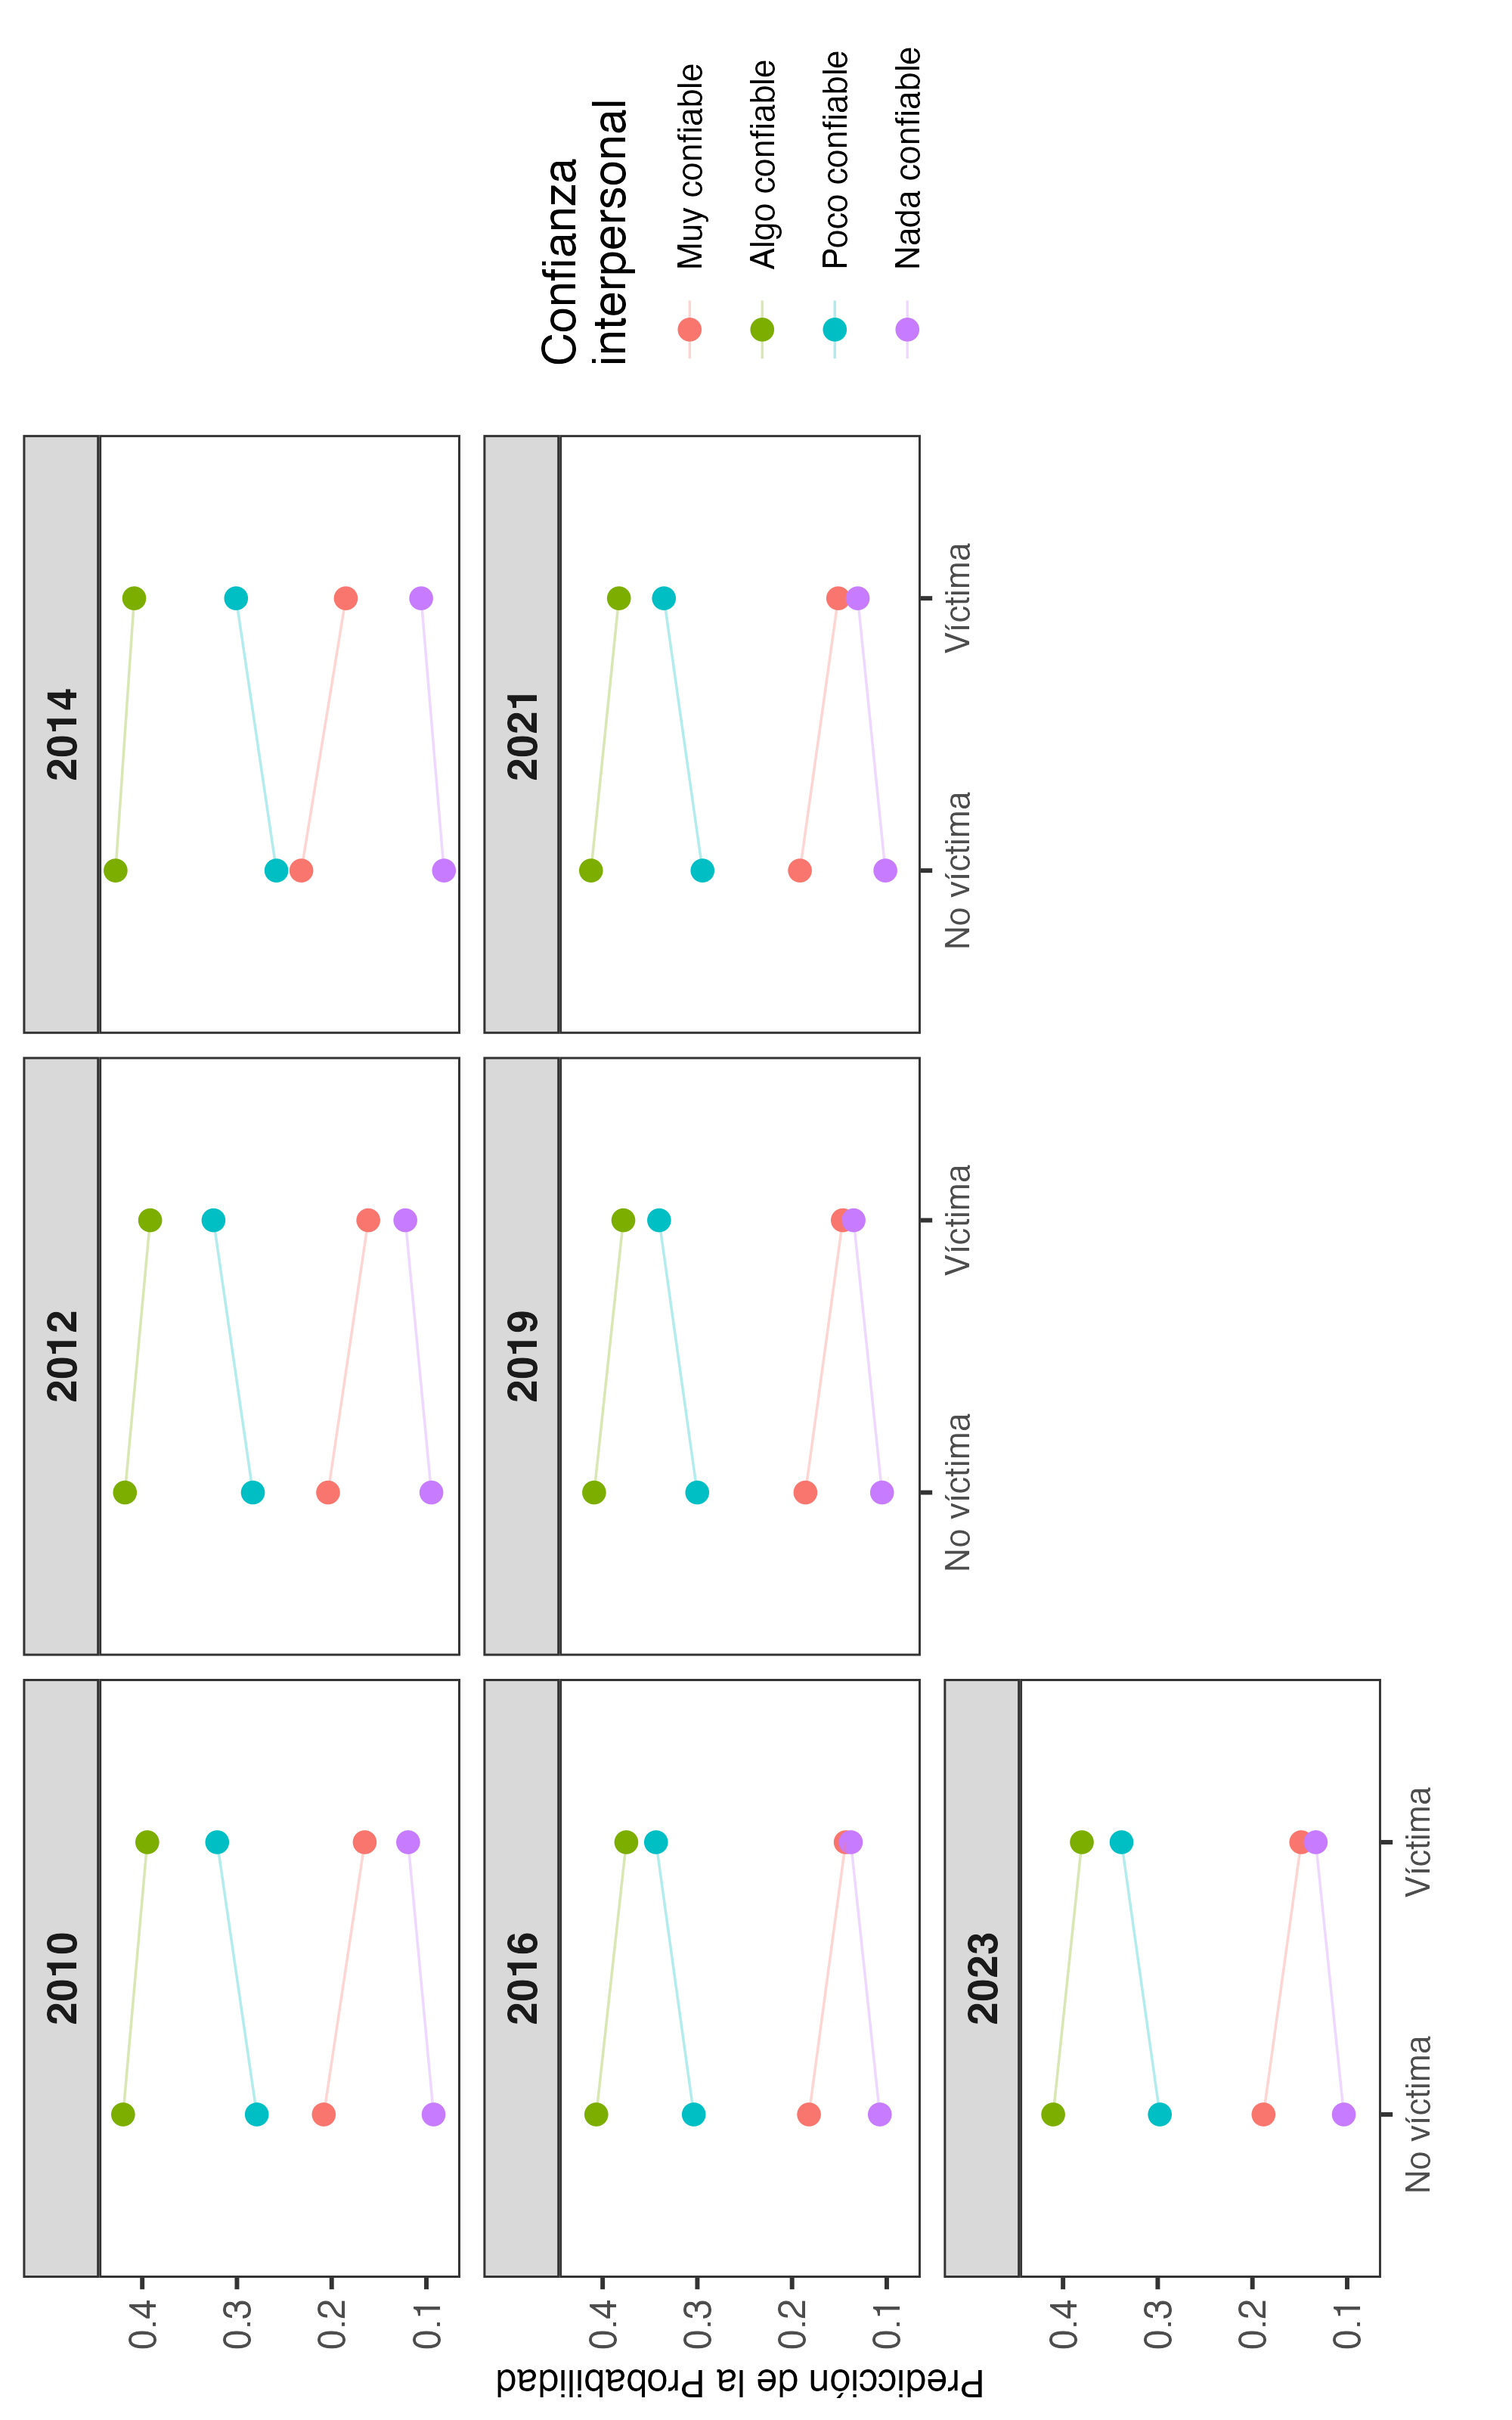
\includegraphics[width = 13cm]{plot_peer_03.png}
    \label{tab:plot5}
\end{center}

\newpage

\begin{center}
Relación entre satisfacción con la democracia y victimización.
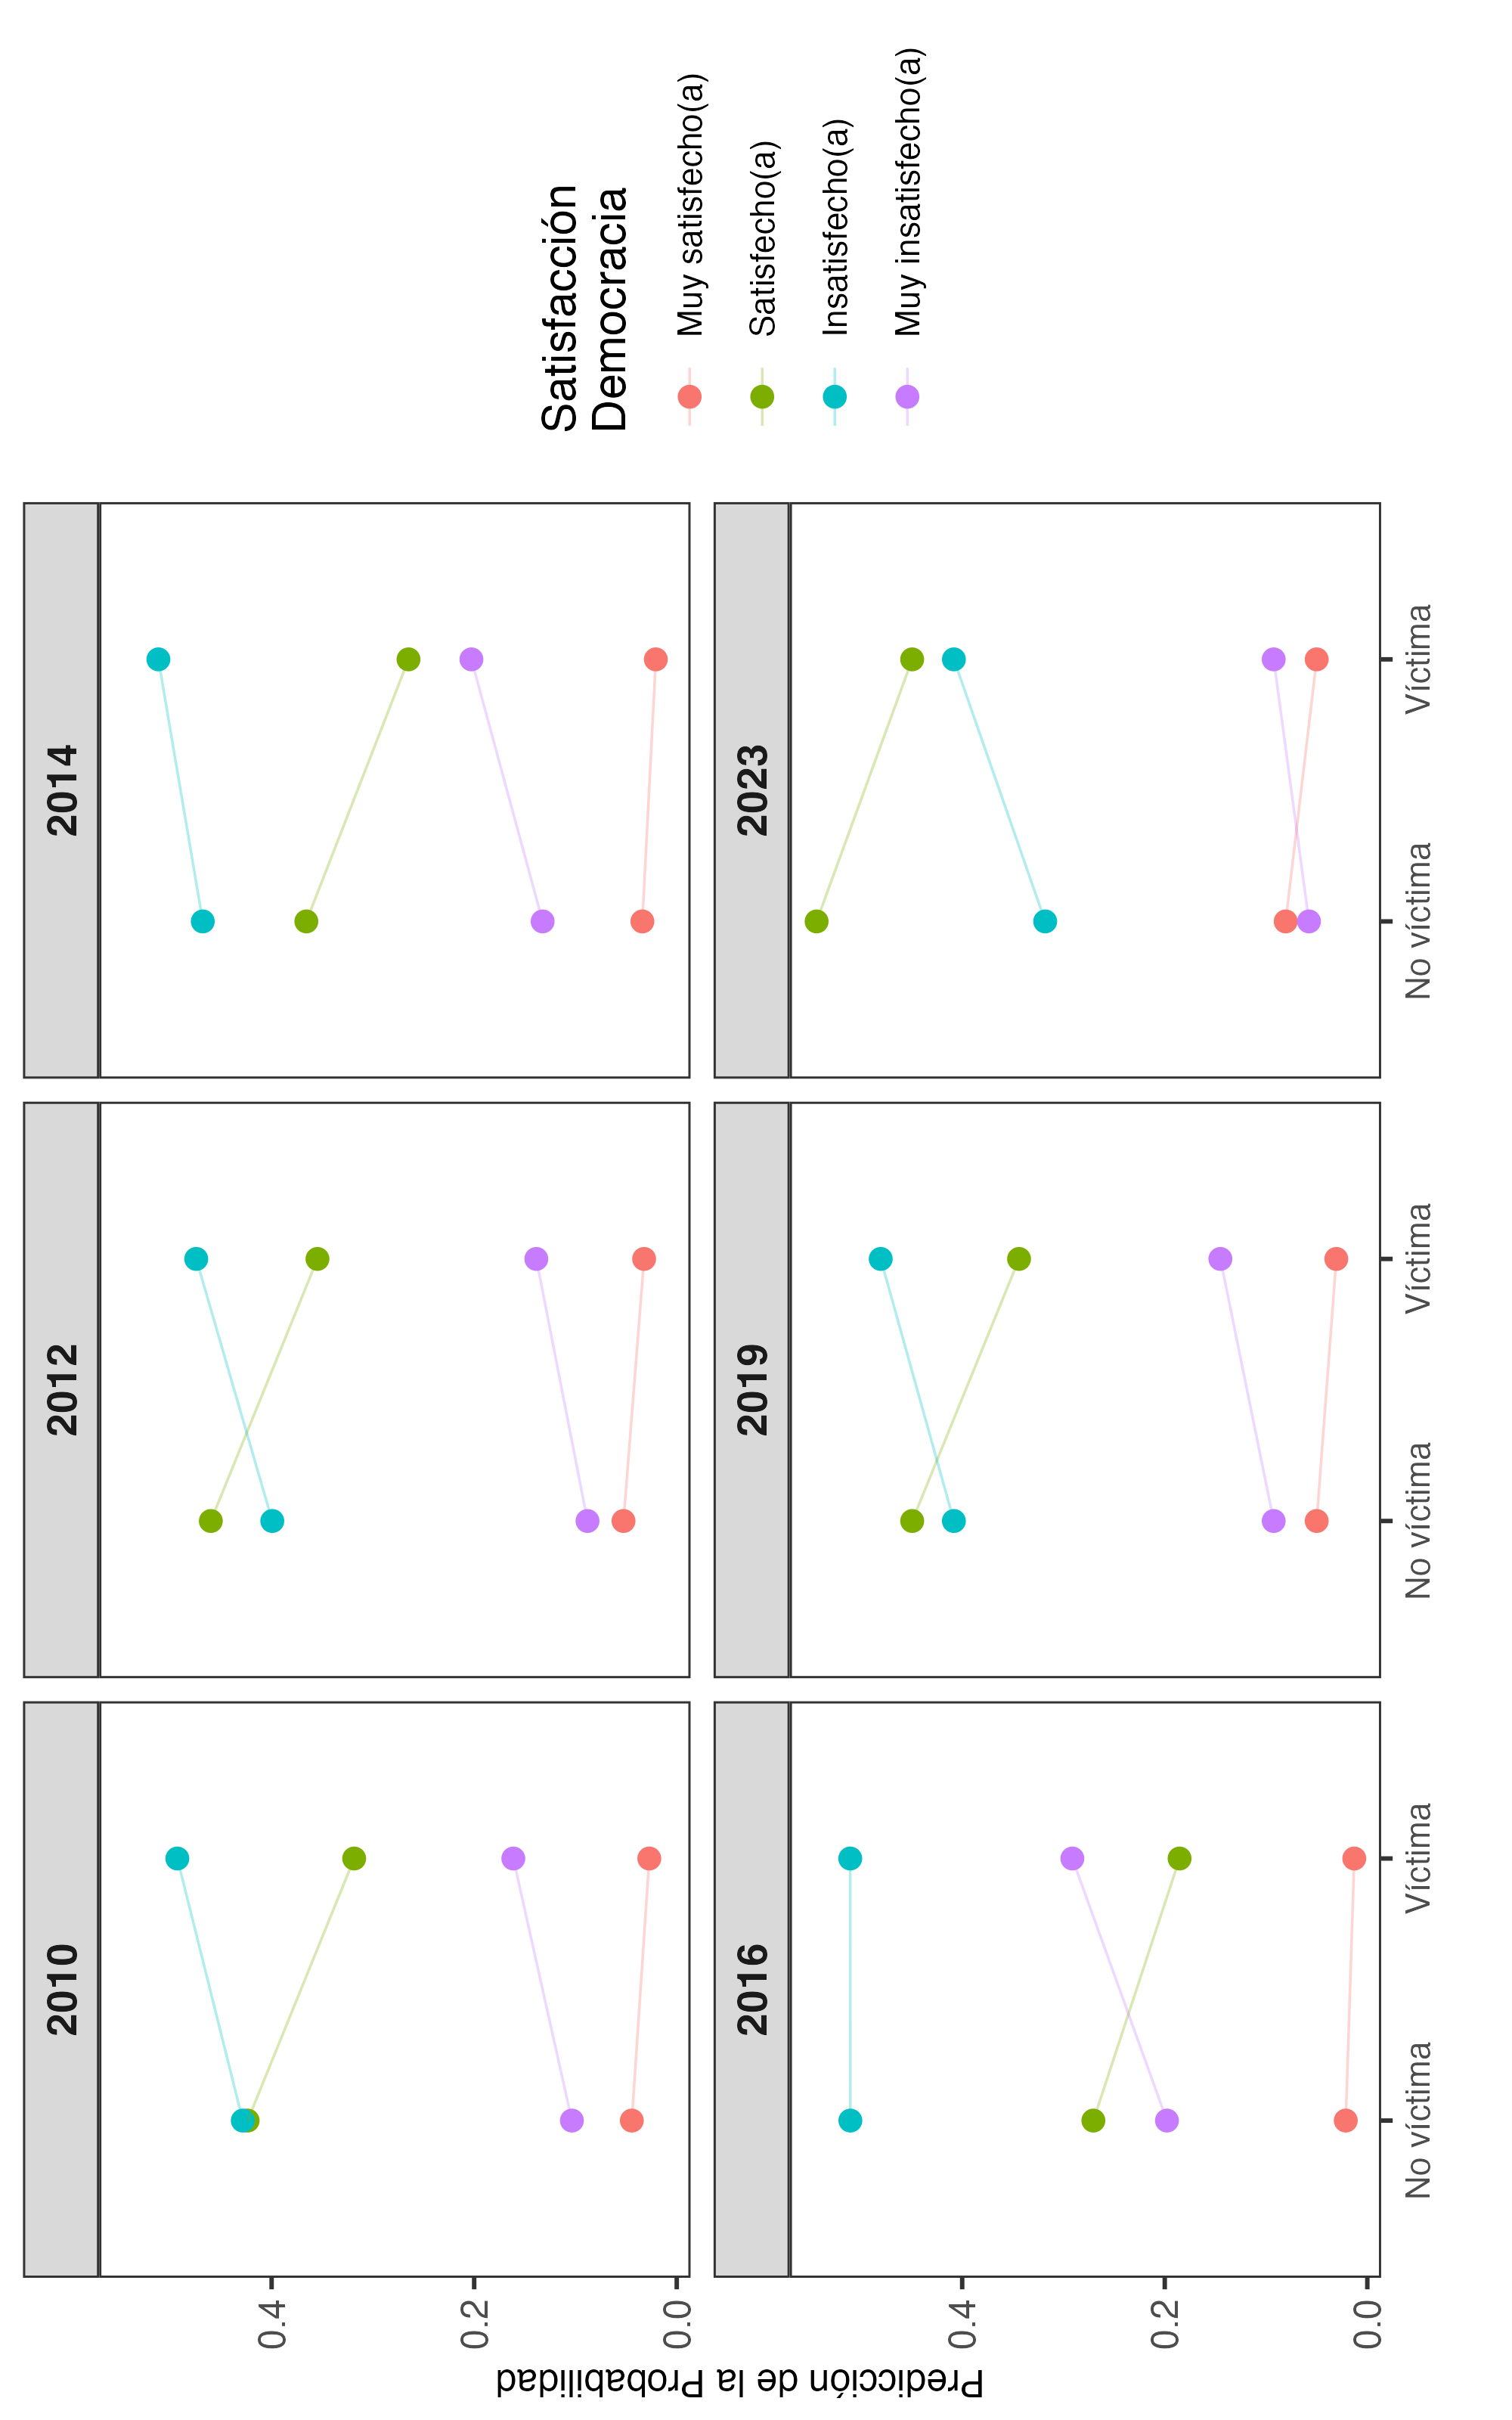
\includegraphics[width = 13cm]{plot_dem_03.png}
    \label{tab:plot6}
\end{center}

\newpage

\begin{center}
Relación entre confianza en el Ejecutivo Federal y victimización.
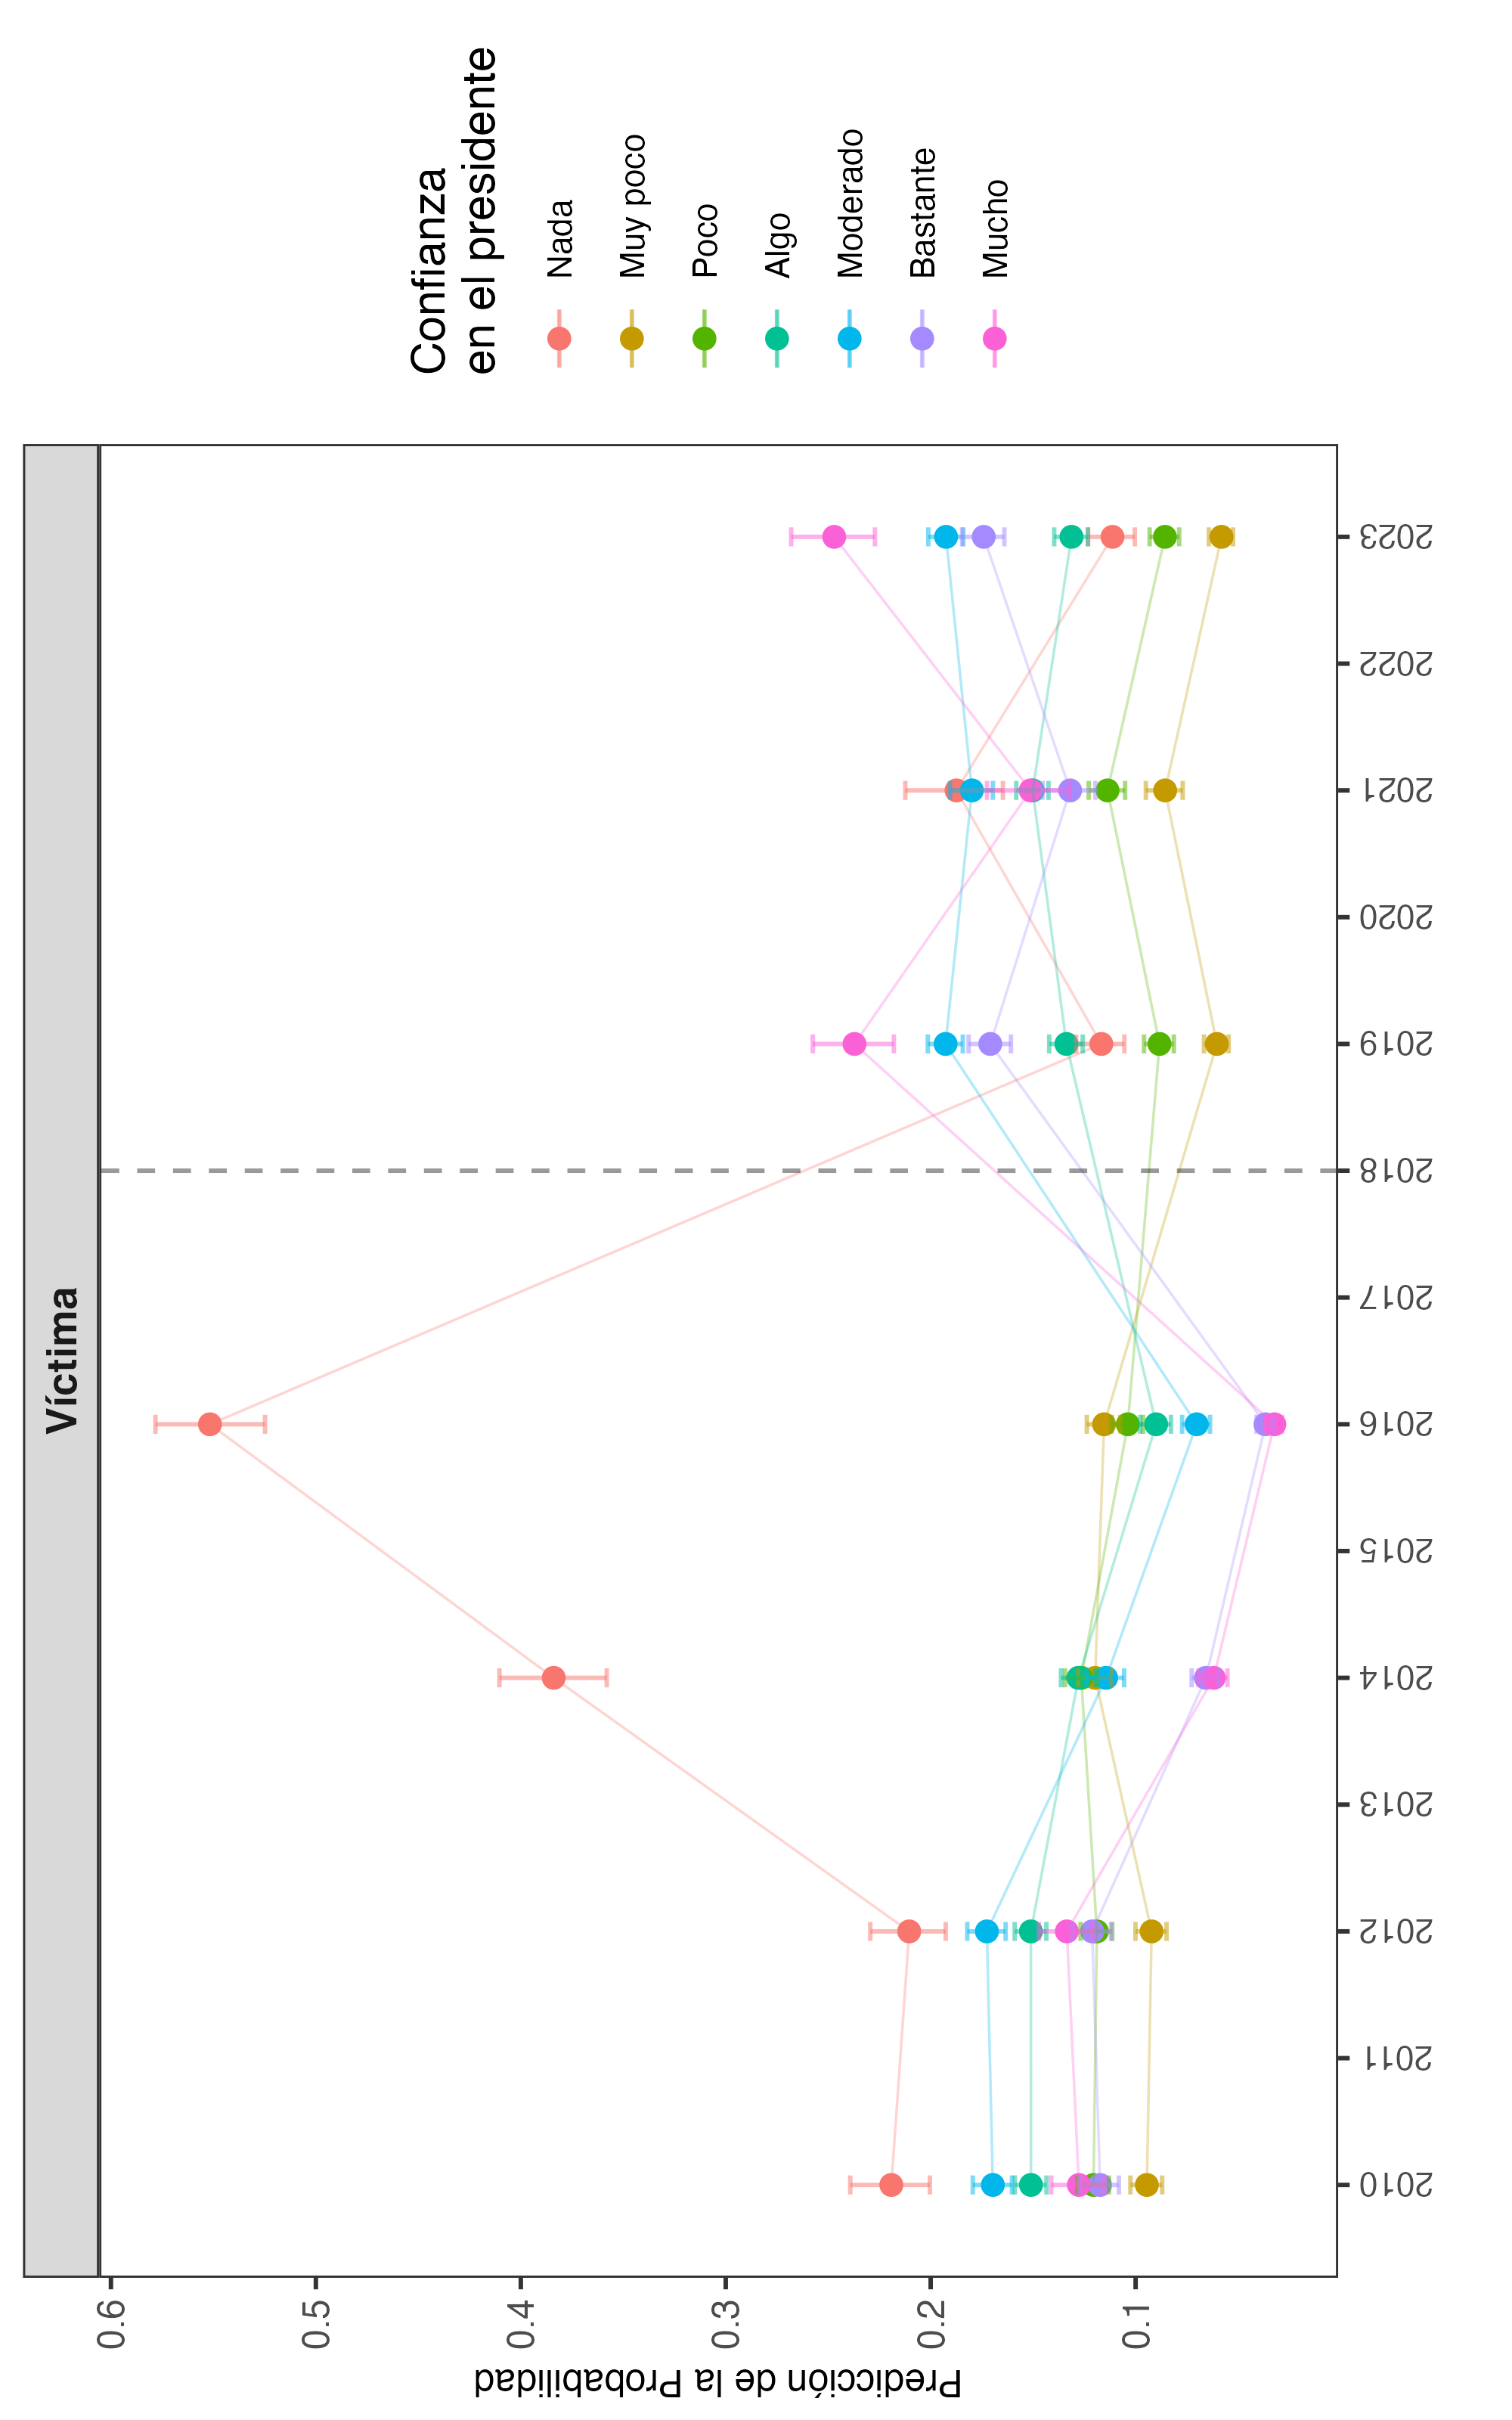
\includegraphics[width = 13cm]{plot_pres_02.png}
    \label{tab:plot3}
\end{center}

\newpage

\begin{center}
Relación entre confianza en la municipalidad y victimización.
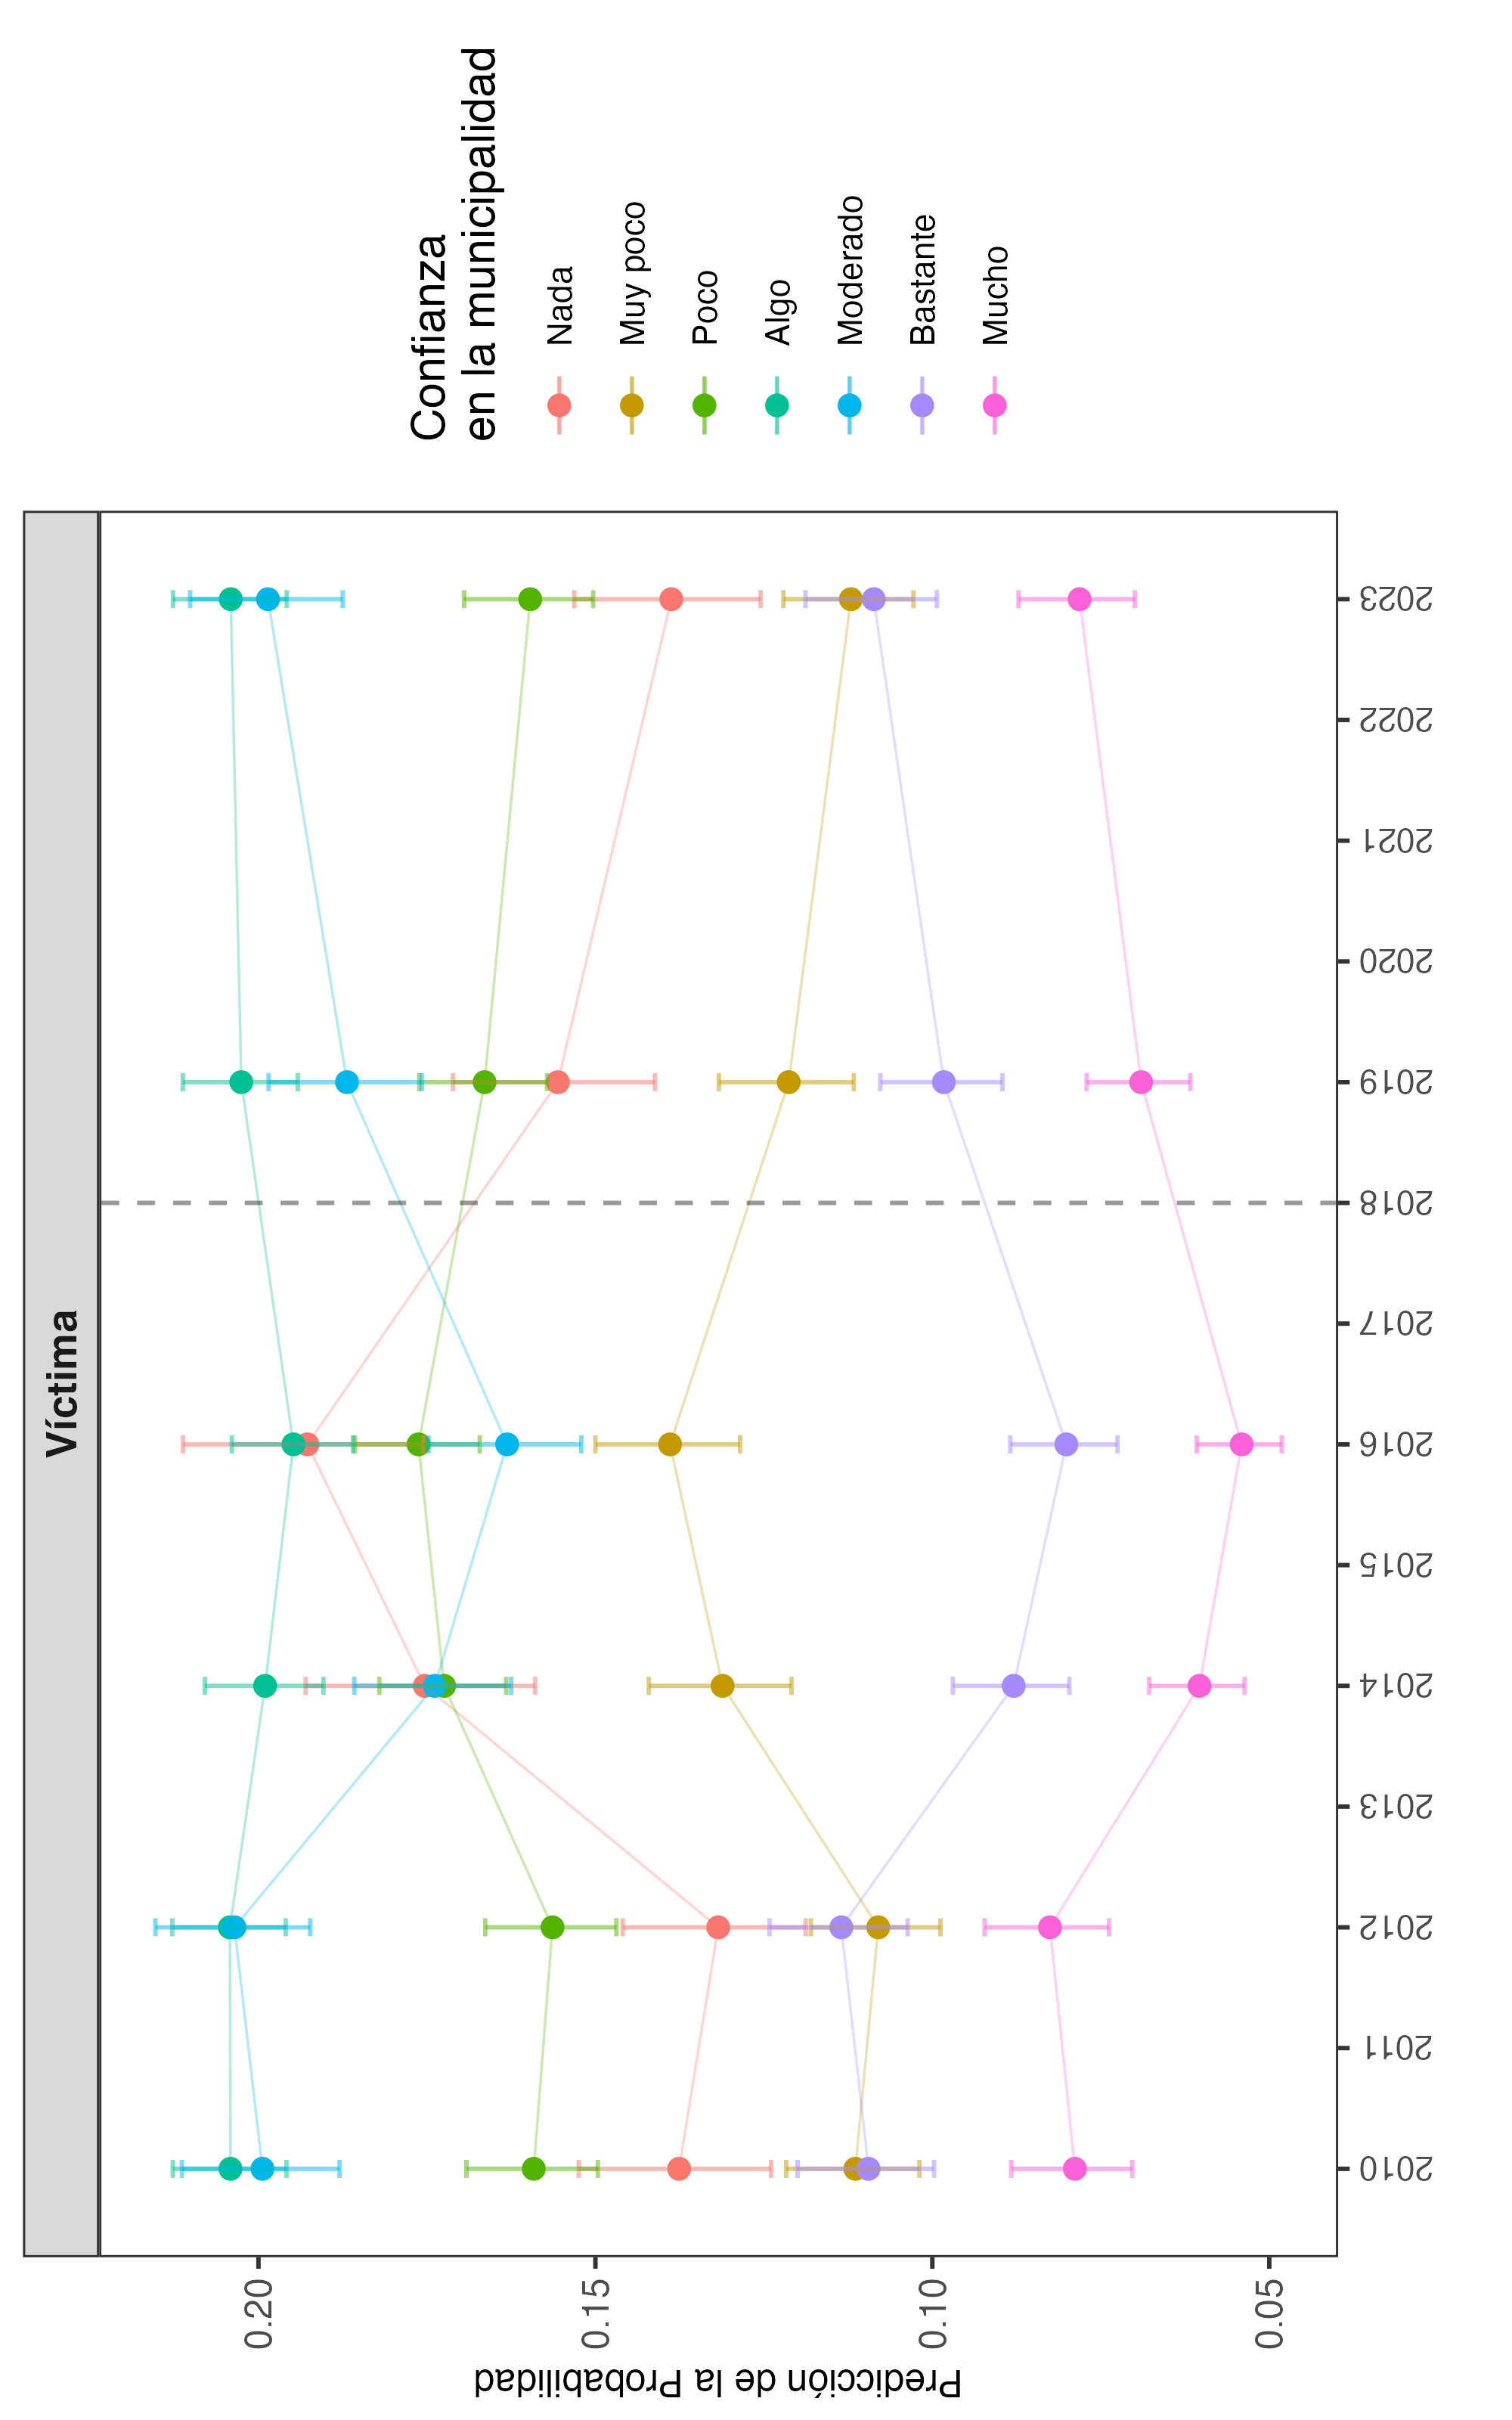
\includegraphics[width = 13cm]{plot_mun_02.png}
    \label{tab:plot4}
\end{center}

\newpage

\begin{center}
Relación entre confianza interpersonal y victimización.
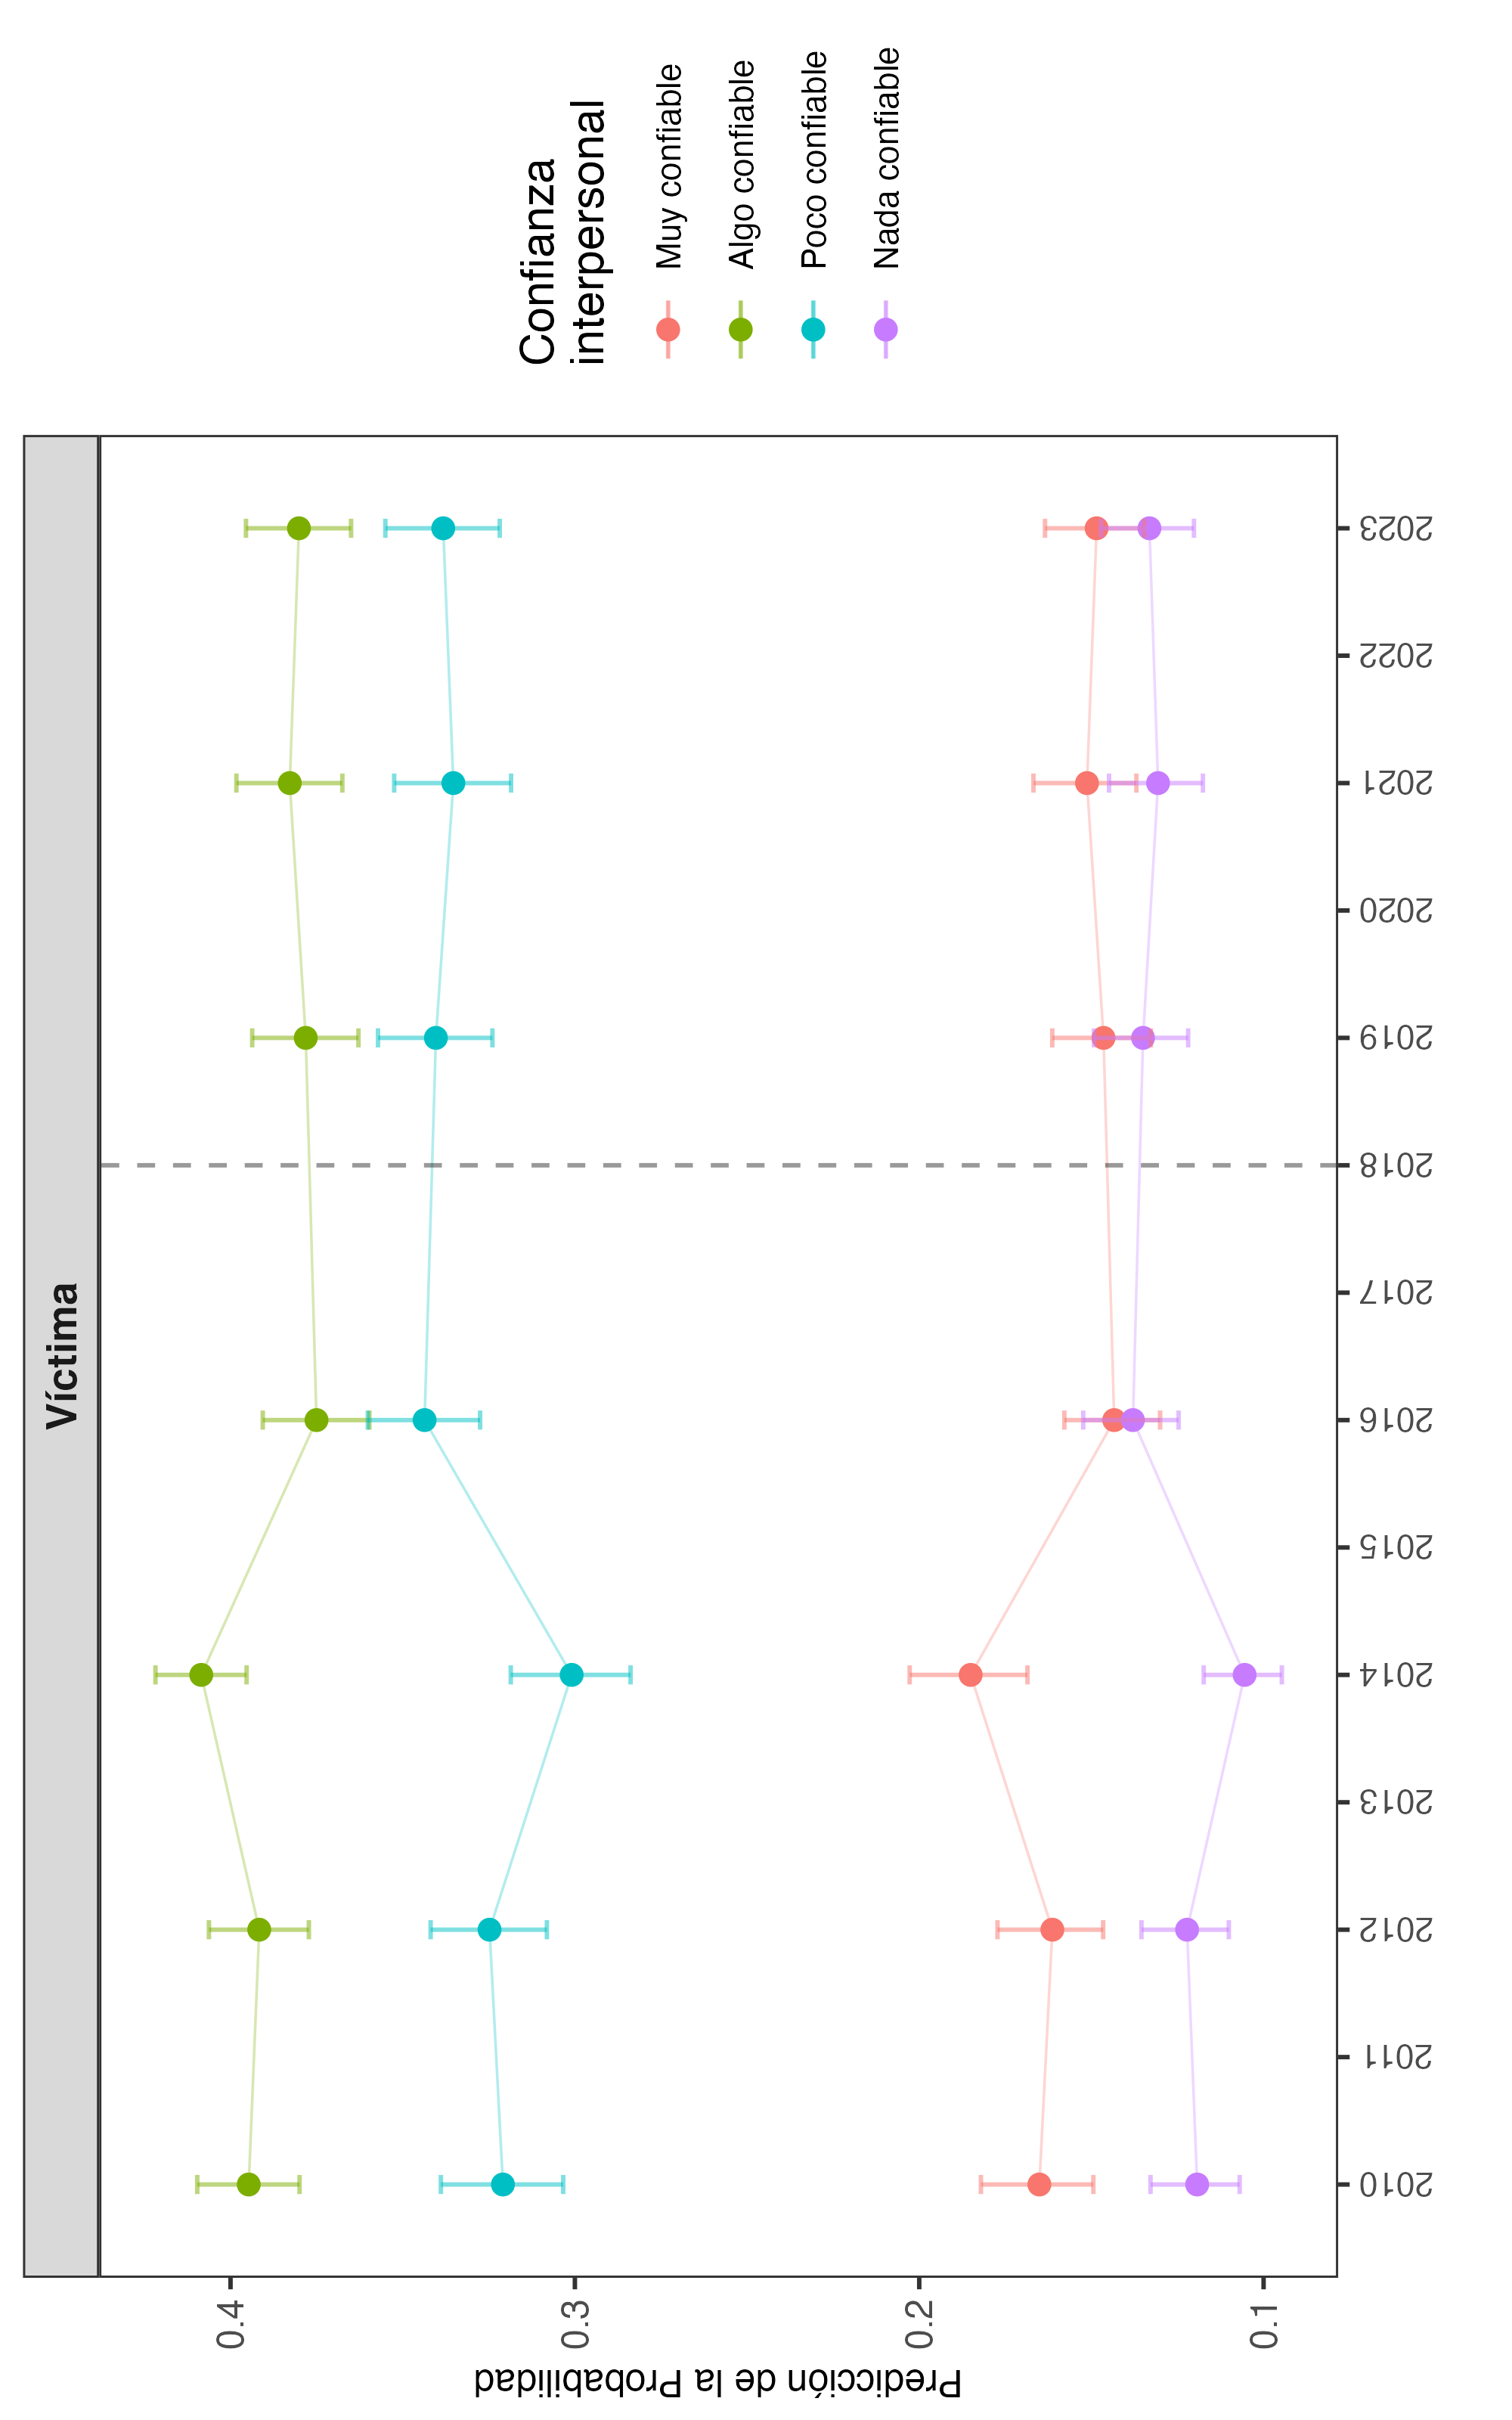
\includegraphics[width = 13cm]{plot_peer_02.png}
    \label{tab:plot5}
\end{center}

\newpage

\begin{center}
Relación entre satisfacción con la democracia y victimización.
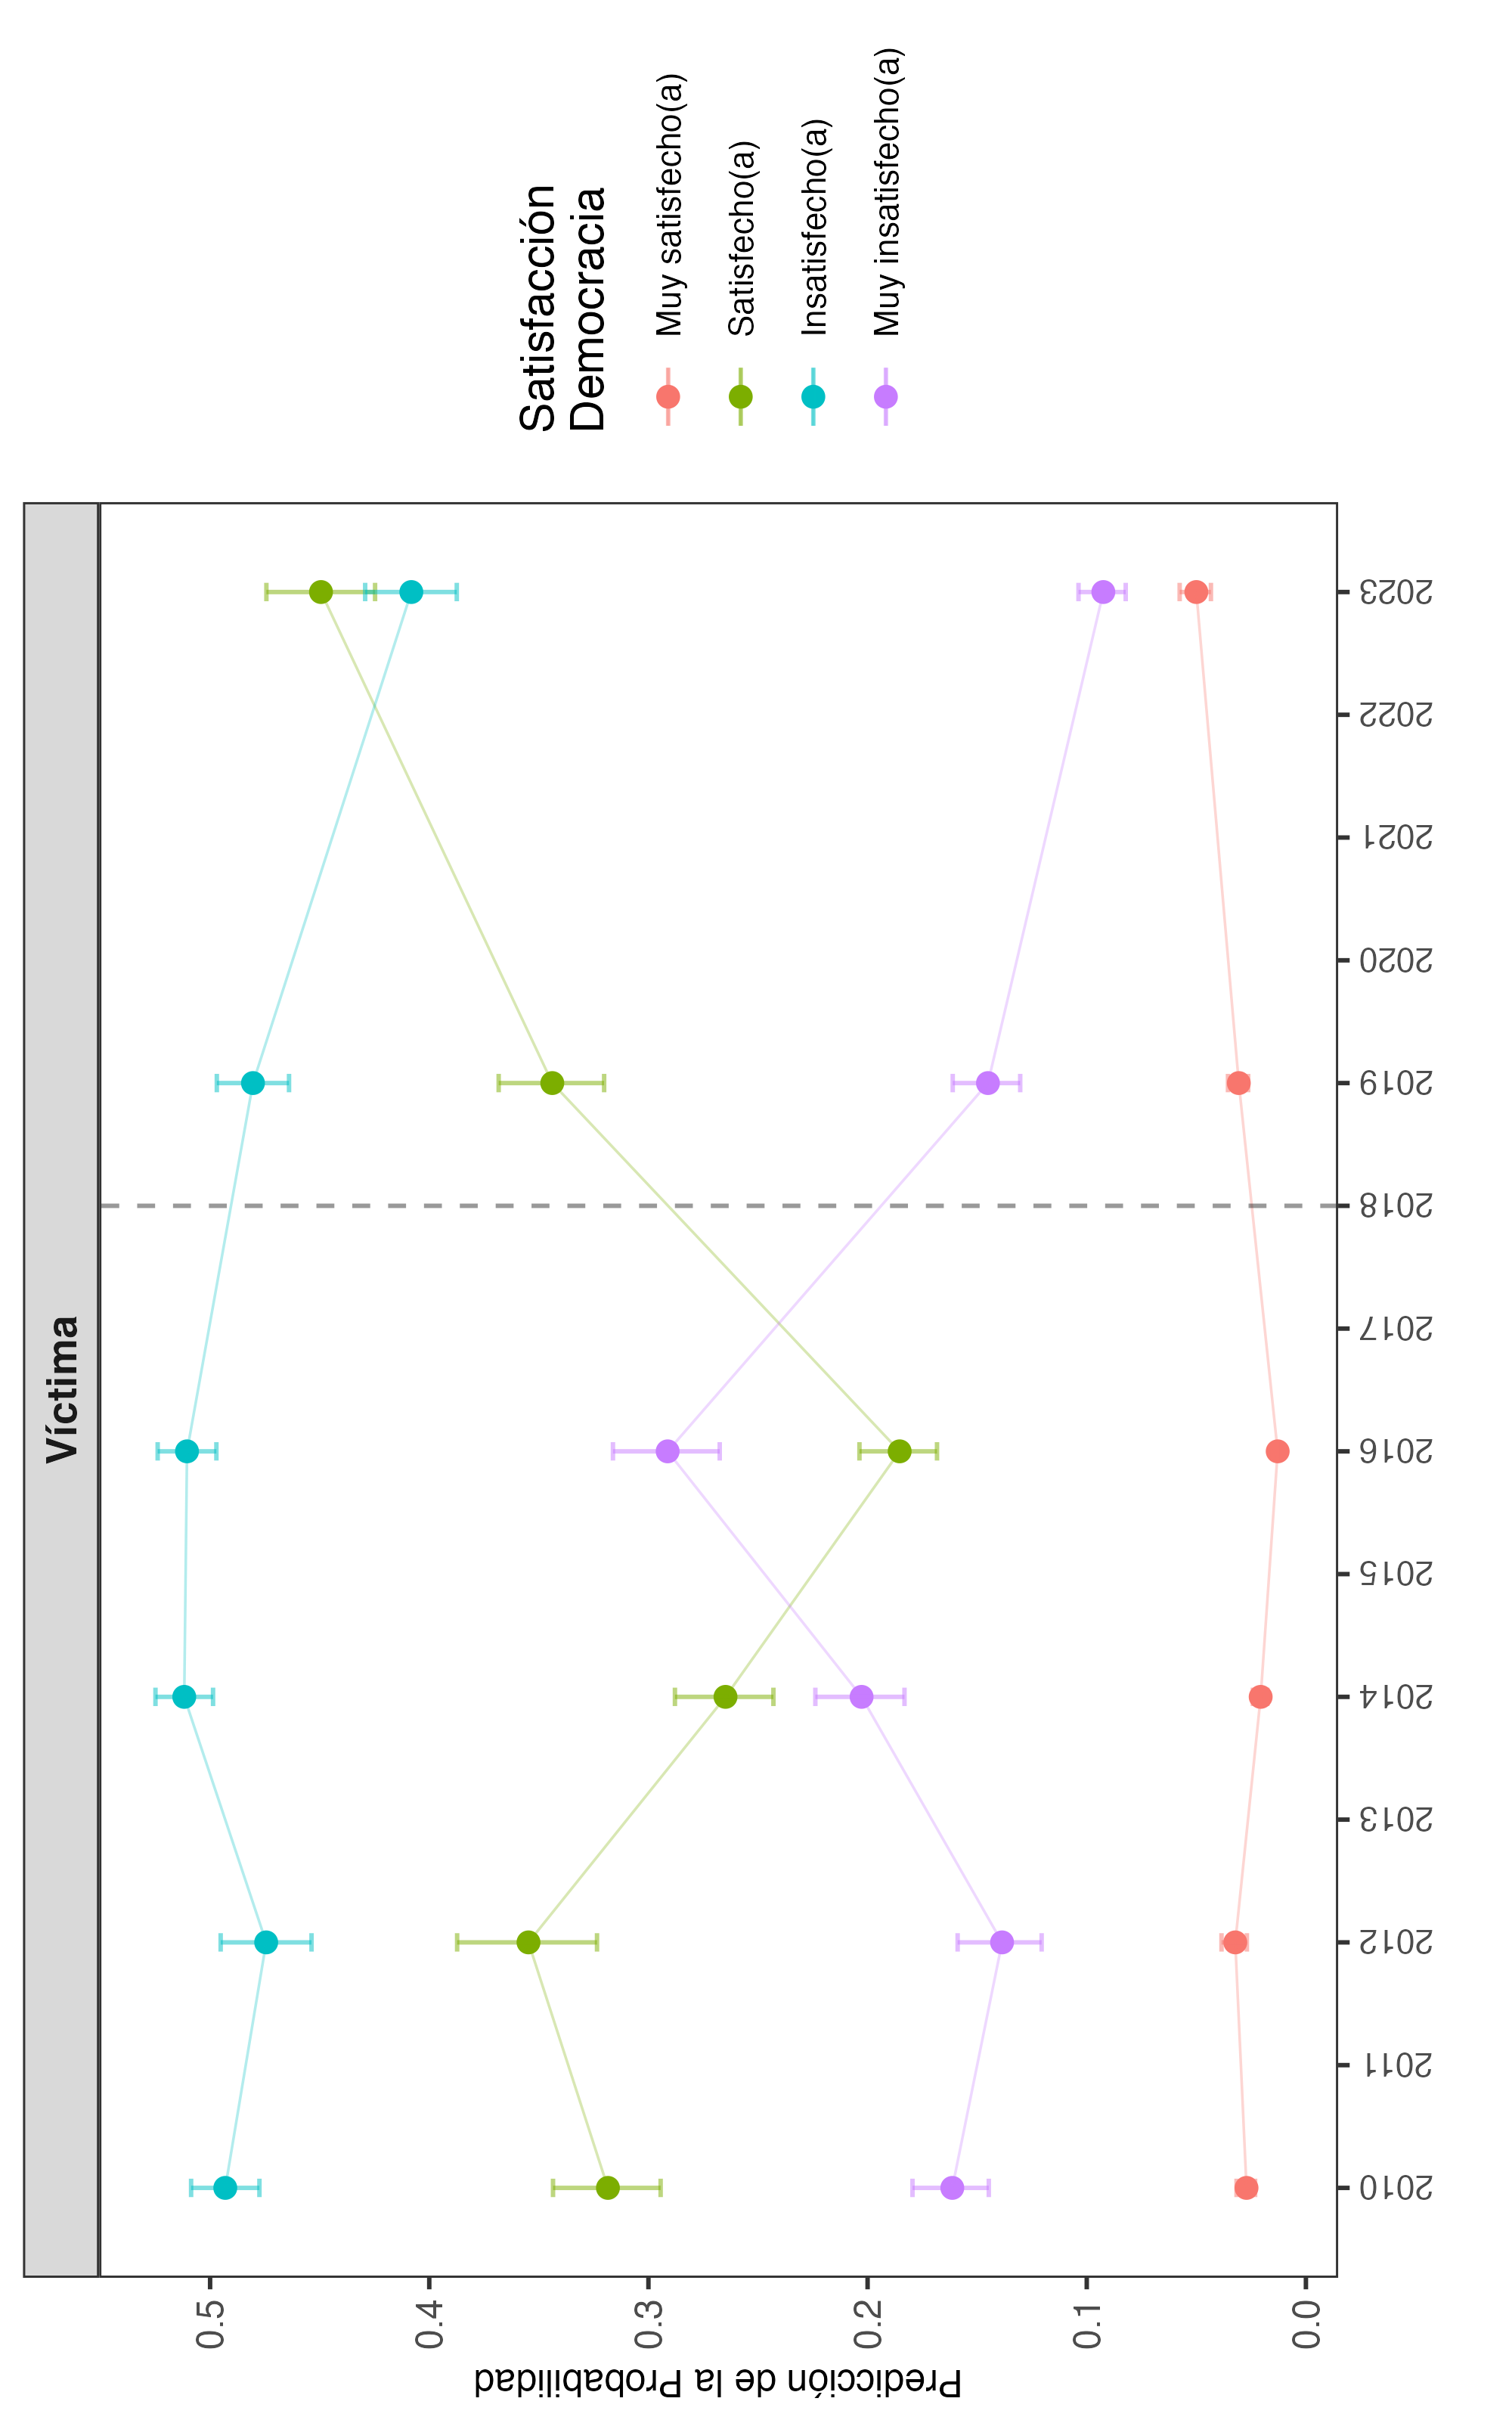
\includegraphics[width = 13cm]{plot_dem_02.png}
    \label{tab:plot6}
\end{center}

\vspace{-0.4cm}

%%%%%%%%
\section{Bibliografía}

\vspace{0.1cm}

\printbibliography[heading = none]

\end{document}